\documentclass[11pt,magyar,a4paper,twoside,]{report}
\usepackage[T1]{fontenc}
\usepackage{ae}
\usepackage{lmodern}
\usepackage{amssymb}
\usepackage{amsmath}
\usepackage{ifxetex,ifluatex}
\usepackage{fixltx2e} % provides \textsubscript
\usepackage{adjustbox}
\usepackage[thmmarks]{ntheorem}
\usepackage{listings}
\usepackage{color}
\usepackage{lastpage}
\usepackage{anysize}
\usepackage{longtable}
\usepackage{sectsty}
\usepackage{setspace}
\usepackage[hang]{caption}
\usepackage{tabularx}
\usepackage{hyphenat}
\usepackage{enumitem}
\usepackage{subcaption}
\usepackage{todonotes}
\usepackage{adjustbox}
\usepackage{minibox}
\usepackage{pdfpages}
\usepackage{tikz}
\usepackage{float}
% fix for pandoc 1.14
\providecommand{\tightlist}{%
  \setlength{\itemsep}{0pt}\setlength{\parskip}{0pt}}
% use microtype if available
\IfFileExists{microtype.sty}{\usepackage{microtype}}{}
% use upquote if available, for straight quotes in verbatim environments
\IfFileExists{upquote.sty}{\usepackage{upquote}}{}
\ifnum 0\ifxetex 1\fi\ifluatex 1\fi=0 % if pdftex
  \usepackage[utf8]{inputenc}
\else % if luatex or xelatex
  \usepackage{fontspec}
  \ifxetex
    \usepackage{xltxtra,xunicode}
  \fi
  \defaultfontfeatures{Mapping=tex-text,Scale=MatchLowercase}
  \newcommand{\euro}{€}
\fi
\usepackage{natbib}
\bibliographystyle{plain}
\usepackage{graphicx}
% We will generate all images so they have a width \maxwidth. This means
% that they will get their normal width if they fit onto the page, but
% are scaled down if they would overflow the margins.
\makeatletter
\def\maxwidth{\ifdim\Gin@nat@width>\linewidth\linewidth
\else\Gin@nat@width\fi}
\makeatother
\let\Oldincludegraphics\includegraphics
%\renewcommand{\includegraphics}[1]{\Oldincludegraphics[scale=1.0]{#1}}
\renewcommand{\includegraphics}[1]{
\begin{adjustbox}{max size={\textwidth}{\textheight}}
    \Oldincludegraphics[scale=0.6]{#1}%
\end{adjustbox}
}
\ifxetex
  \usepackage[setpagesize=false, % page size defined by xetex
              unicode=false, % unicode breaks when used with xetex
              xetex]{hyperref}
\else
  \usepackage[unicode=true]{hyperref}
\fi
\definecolor{darkgreen}{rgb}{0,0.5,0}
\hypersetup{breaklinks=true,
            bookmarks=true,
            pdfauthor={},
            pdftitle={},
            colorlinks=true,
            urlcolor=blue,
            linkcolor=magenta,
            citecolor=darkgreen,
            pdfborder={0 0 0}}
\urlstyle{same}  % don't use monospace font for urls
\setlength{\parindent}{0pt}
\setlength{\parskip}{6pt plus 2pt minus 1pt}
\setlength{\emergencystretch}{3em}  % prevent overfull lines
\ifxetex
  \usepackage{polyglossia}
  \setmainlanguage{}
\else
  \usepackage[magyar]{babel}
\fi

\title{Mikroszolgáltatás alapú architektúra fejlesztésének és tesztelésének támogatása}
\author{Borlay Dániel}

\renewcommand*{\hyperref}[2][\ar]{%
  \def\ar{#2}
  #2 (\refstruc{#1})}

\renewcommand*{\figureautorefname}{ábra}

\sloppy

% for English documents
%\setlength{\parindent}{0pt} % áttekinthetőbb, angol nyelvű dokumentumokban jellemző
%\setlength{\parskip}{8pt plus 3pt minus 3pt} % áttekinthetőbb, angol nyelvű dokumentumokban jellemző

% for Hungarian documents
\setlength{\parindent}{12pt}
\setlength{\parskip}{0pt}

\marginsize{35mm}{25mm}{15mm}{15mm} % anysize package
\setcounter{secnumdepth}{0}
\sectionfont{\large\upshape\bfseries}
\setcounter{secnumdepth}{3}
\singlespacing
\frenchspacing


\begin{document}

\footnotesize


\normalsize

%--------------------------------------------------------------------------------------
% The title page
%--------------------------------------------------------------------------------------
\begin{titlepage}
\begin{center}
\Oldincludegraphics[width=60mm,keepaspectratio]{img/BME1782logo.pdf}\\

\vspace{0.3cm}
\textbf{Budapesti Műszaki és Gazdaságtudományi Egyetem}\\
\textmd{Méréstechnika és Információs Rendszerek Tanszék}\\
\textmd{}\\[5cm]

\vspace{0.4cm}
{\huge \bfseries Mikroszolgáltatás alapú architektúra fejlesztésének és tesztelésének támogatása}\\[0.8cm]
\vspace{0.5cm}
\textsc{\Large Diplomaterv}\\[4cm]

\begin{tabular}{cc}
 \makebox[7cm]{\emph{Készítette}} & \makebox[7cm]{\emph{Konzulens}} \\
 \makebox[7cm]{Borlay Dániel} & \makebox[7cm]{Szatmári Zoltán}
\end{tabular}

\vfill
{\large \today}
\end{center}
\end{titlepage}

\onehalfspacing

\hypersetup{linkcolor=black}
\setcounter{tocdepth}{2}
\tableofcontents

\vfill
\clearpage

\begin{center}
\large
\textbf{HALLGATÓI NYILATKOZAT}\\
\end{center}

Alulírott \emph{Borlay Dániel}, szigorló hallgató kijelentem, hogy ezt a diplomatervet meg nem engedett segítség nélkül, saját magam készítettem, csak a megadott forrásokat (szakirodalom, eszközök stb.) használtam fel. Minden olyan részt, melyet szó szerint, vagy azonos értelemben, de átfogalmazva más forrásból átvettem, egyértelműen, a forrás megadásával megjelöltem.

Hozzájárulok, hogy a jelen munkám alapadatait (szerző(k), cím, angol és magyar nyelvű tartalmi kivonat, készítés éve, konzulens(ek) neve) a BME VIK nyilvánosan hozzáférhető elektronikus formában, a munka teljes szövegét pedig az egyetem belső hálózatán keresztül (vagy autentikált felhasználók számára) közzétegye. Kijelentem, hogy a benyújtott munka és annak elektronikus verziója megegyezik. Dékáni engedéllyel titkosított diplomatervek esetén a dolgozat szövege csak 3 év eltelte után válik hozzáférhetővé.

\begin{flushleft}
\vspace*{1cm}
Budapest, \today
\end{flushleft}

\begin{flushright}
 \vspace*{1cm}
 \makebox[7cm]{\rule{6cm}{.4pt}}\\
 \makebox[7cm]{\emph{Borlay Dániel}}\\
 \makebox[7cm]{hallgató}
\end{flushright}
\thispagestyle{empty}

\vfill
\clearpage
\thispagestyle{empty} % an empty page

\chapter*{Kivonat}\label{kivonat}
\addcontentsline{toc}{chapter}{Kivonat}

Napjainkban komoly gondot okoz, hogy hogyan lehet hatékonyan elosztott,
jó rendelkezésre állású, könnyen skálázható alkalmazást építeni. Sok
architektúrális megközelítés van, amit alapul véve hatékonyan
tervezhetjük meg a rendszerünket, és könnyen elkészíthetjük az
alkalmazásunkat. Egy ilyen architektúrális megközelítés a
mikroszolgáltatásokon alapuló architektúra, amivel apró részletekre
bontva a feladatot, könnyen kezünkben tarthatjuk az elosztott
alkalmazásunkat.

A mikroszolgáltatásokra épülő architekrúra (microservices), egy olyan
architektúrális fejlesztési módszertan, ami a programot alkotóelemeire
szedi, és minden funkcionalitást teljesen különálló egységként kezel.
Egy ilyen alkalmazás fejlesztése közben oda kell figyelni az összes
szolgáltatással való együttműködésre, a visszamenőleges
kompatibilitásra, és meg kell tartani az alkotóelemek kapcsolatának a
konzisztenciáját. Ennek a fenntartása egy nehéz feladat, amit kézileg
szinte lehetetlen hosszú távon fenntartani.

A diplomamunka keretében az volt a feladatom, hogy megismerjem az
architektúra lényegét és működését, illetve kiderítsem, hogy milyen
eszközökkel tudom automatizálás segítségével támogatni a fejlesztés, és
működtetés folyamatát.

A diplomamunka célkitűzése, hogy egy olyan mikroszolgáltatásokra épülő
alkalmazást készítsek, amellyel be tudom mutatni az architektúra
előnyeit, végig tudom vezetni rajta a tesztelés folyamatát, tudom
automatizálni a tesztelését, és működtetését, és betekintést tudok adni
az architektúrához használatos technológiákba.

\chapter*{Abstract}\label{abstract}
\addcontentsline{toc}{chapter}{Abstract}

Nowadays it's a very big problem, that how to build a distributed,
highly available, easily scalable application efficiently. There are
many ways to design our system, which tells how we can implement our
application efficiently. One of these design patterns is the
microservice based architecture, which creates small services from the
big application, by separating the functionality, and we can handle more
efficiently our distributed application.

Microservice architecture is a software development methodology, which
separates the parts of the application to the smallest functionality,
which could be run from a separated environment. It is important to take
care about the cooperation between the services, the backward
compatibility and the consistency of the service connectivity through
the development flow. It is hard to keep these attributes, and almost
impossible to keep it on long term by manual verification.

In this thesis I gathered knowledge about the architecture, how it
works, how it could be designed, or which continuous integration tool
could be used for helping development and maintenance.

The goal of this thesis is to create and example application based on
microservice architecture, which could be used for showing the
advantages of the technique, and I can show the full process of testing
and design. My goal also to create a framework for helping the
development of the application by automated testing and integration.

\chapter{Bevezetés}\label{bevezetuxe9s}

A mai informatikai nagyvállalatok rengeteg egymástól különböző
alkalmazást készítenek. Minden alkalmazás fejlesztése és karbantartása
nagy feladatot jelent, mivel rengeteg emberi erőt emészt fel a fordítás,
telepítés, és a tesztelés. Sok hiba forrását jelenti a kézileg
végrehajtott munkafolyamat, és a fejlesztőkre van bízva, hogy mely
teszteket akarják futtatni a saját programjukon, és figyelmen kívül
hagyhatják a más alkalmazásokkal történő egymásra hatásokat. A cég
számára nagy költség lehet az ebből fakadó problémák kiküszöbölése, és
ellenőrzése, illetve hatalmas adminisztrációs problémát okozhat.

A fejlesztők nem mindig képzettek, és nem is feltétlenül a feladatuk a
tesztelés, így felesleges erőforrásokat vesz el a kézi tesztelés, és a
telepítés ami a tesztek futtatásához kellhet. Orvosolható ez a probléma
képzett tesztelők felvételével, de ez többlet költségeket okoz. Könnyen
lehet az is a probléma, hogy a tesztelés nem elég teljeskörű, és az
alkalmazásból nem lesz minden komponens kitesztelve, illetve az elemek
közötti kapcsolat változtatása előzetes figyelmeztetés nélkül érvényre
kerülhet. Ezzel rejtett hibákat hagyhatunk az alkalmazásban, amiket
később komoly erőforrások, és költségek árán lehet csak kijavítani. Ha
nem nézzük meg, hogy az alkalmazás minden egyes része jól működik-e
együtt, akkor olyan hibákat hagyhatunk a rendszerben, amit nagyon
nehezen lehet detektálni, és még nehezebb felelősöket hozzárendelni.
Ahhoz, hogy ezeket a problémákat kiküszöböljük egy jól definiált
tesztelési módszerre van szükség, amit be kell tartatni, illetve az
alkalmazás részeit egy környezetbe telepítve kell egyszerre tesztelni,
mivel így teljeskörűen vizsgálható a termék. Ha nincs felügyelve a
teljes munkafolyamat, akkor olyan információk is elveszhetnek, mint a
fordítással, vagy a telepítéssel kapcsolatos információk, ami sokat
segíthet egy hiba feltárása során.

Nagy segítséget nyújthat egy automatizált keretrendszer, amelynek a
célja, hogy levegye a terhet a fejlesztő válláról, és jól definiált
módon hajtsa végre a fejlesztést, telepítést, és tesztelést. Az
automatizálatlan fejlesztési fázisok potenciális veszélyforrások a
végeredmény szempontjából, és a követhetőségük, reprodukálhatóságuk, és
rugalmasságuk is sokkal rosszabb. Erre a problémára nyújt megoldást a
folytonos integráció (Continuous Integration), illetve a folytonos
telepítés (Continuous Deployment), mely módszertanok megmondják, hogy
hogyan, és milyen módszerekkel lehet elősegíteni a jól végrehajtott, és
ellenőrzött fejlesztési folyamatot. Egy folytonos integrációt támogató
rendszerben minden folyamat felügyelt módon hajtódik végre, és pontosan
azokat a lépéseket hajtja végre amit előzetesen definiáltak neki, így
egyszerűsíti az adminisztrációt, növeli a tesztlefedettséget minden
részegységre, és figyelembe veszi a teljes alkalmazás részenkénti
egyűttműködését, mindezt automatizáltam, a fejlesztő beavatkozása
nélkül.

Jelen diplomamunka célja, hogy bemutassam a mikroszolgáltatások
architektúrára épülő alkalmazások előnyeit, hátrányait, és fejlesztésük
folyamatát, az ilyen alkalmazásokhoz tartozó legjellemzőbb
technológiákat, és elkészítési stratégiákat. Meg kell terveznem és el
kell készítenem egy folytonos integrációt támogató keretrendszert, ami
képes a mikroszolgáltatásokhoz tartozó feladatok mind elemi, mind teljes
architektúra szempontjából való ellenőrzésére, illetve értékelnem kell
az elkészült keretrendszert a minta alkalmazás segítségével.

A diplomamunka keretében elkészítettem egy könyvesbolt webes felületét
kiszolgáló minta alkalmazást, amely a mikroszolgáltatások architektúrára
épült, és készítettem egy ennek a fejlesztését, és tesztelését támogató
folytonos integráción alapuló keretrendszert, ami képes az alkalmazás
minden részletét fordítani, telepíteni, és tesztelni. A minta alkalmazás
elkészítése közben figyeltem a funkciók szerinti szétbontásra, és a
szolgáltatások közötti kommunikáció bővíthető implementációjára. A
folytonos integrációt támogató keretrendszer amit elkészítettem képes
lefordítani az összes szolgáltatás forrásából a telepítéshez szükséges
artifact-okat, és elérhetővé teszi a webes felületen keresztül. Képes a
folytonos telepítésre, vagyis a szolgáltatásokat egymástól függetlenül
telepíteni, és egy működő alkalmazást kialakítani.

A diplomamunka struktúráját tekintve a következő képpen néz ki:

Az második fejezetben beleástam magam a technológiai áttekintésbe, ahol
az architektúra lényegét próbáltam megérteni, és összeszedtem, hogy
milyen tervezési kérdések merülnek fel egy mikroszolgáltatásokra épülő
alkalmazás elkészítésénél. Körüljártam a felhasználható technológiákat,
és megnéztem milyen referencia alkalmazások léteznek a piacon.

A harmadik fejezetben a minta alkalmazást, és a hozzá tartozó folytonos
integrációt támogató keretrendszert terveztem meg. A tervezés közben
kitértem a szolgáltatások különválasztásának okaira, és feladataik
szétosztására, illetve megterveztem a kommunikációt a részek között.
Kifejtettem mit is jelent a folytonos integráció, és hogyan lehet
felhasználni hatékonyan mikroszolgáltatások architektúrára épülő
alkalmazások esetén, majd bemutattam az elkészítendő keretrendszert.

A negyedik fejezetben az implementációt fejtettem ki részleteiben,
kitérve az egyes szolgáltatások megvalósításához kellő logika
elkészítésére, és a környezet előkészítéséhez kellő Docker konténerekre.
Bemutattam a kommunikáció működését, és kitértem a teljes alkalmazás
átfogó felépülésére. A folytonos integrációt támogató keretrendszer
esetében bemutattam a Jenkins eszközt, amit a diplomamunka
elkészítéséhez felhasználtam, illetve az egyes alkotó elemeket mutattam
be részleteiben.

Az ötödik fejezetben értékeltem az elkészített alkalmazást, és
keretrendszert, illetve adtam pár fejlesztési javaslatot, amellyel jobbá
tehető mind az alkalmazás, mint a támogató keretrendszer. Megemlítettem
a fejlesztés közben fellépő hibákat, és elmagyaráztam a megoldásukat.

\chapter{Háttérismeretek}\label{huxe1ttuxe9rismeretek}

\section{Mikroszolgáltatások}\label{mikroszolguxe1ltatuxe1sok}

A mikroszolgáltatások\citep{microservices} \citep{micro-arch}
\citep{microservices-light} egy olyan architektúrális tervezési módszer,
amikor a tervezett rendszert/alkalmazást kisebb funkciókra bontjuk, és
önálló szolgáltatásokként, önálló erőforrásokkal, valamilyen jól
definiált interfészen keresztül tesszük elérhetővé.

Ezt az architektúrális mintát az teszi erőssé, hogy nem függenek
egymástól a különálló komponensek, és csak egy kommunikációs interfészt
ismerve is karbantartható a rendszer. Egy szoftver fejlesztési
projektben előnyös lehet, hogy az egyes csapatok fókuszálhatnak a saját
szolgáltatásukra, és nincs szükség a folyamatos kompatibilitás
tesztelésére.

Egy mikroszolgáltatást használó architektúra kiépítéséhez sokféle
funkcionális elkülönítési módot használnak, amivel a szolgáltatásokat
kialakíthatjuk. Egy ilyen elválasztásí módszer a rendszer
specifikációjában lévő főnevek vagy igék kiválasztása, és az így kapott
halmaz felbontása. Egy felbontás akkor minősül ideálisnak, ha nem tudjuk
tovább bontani az adott funkciót. A valóságban soha nem lesz az
ideálisnak megfelelő felbontás, mivel erőforrás pazarló, és túlzottan
elosztott rendszert kapnánk.

\subsection{\texorpdfstring{Szolgáltatás elválasztás
tervezése\label{splitting}}{Szolgáltatás elválasztás tervezése}}\label{szolguxe1ltatuxe1s-elvuxe1lasztuxe1s-tervezuxe9se}

A tervezési folyamatnál a következő szempontokat szokták figyelembe
venni:

\begin{itemize}
\tightlist
\item
  Szolgáltatások felsorolása valamilyen szempont szerint

  \begin{itemize}
  \tightlist
  \item
    Lehetséges műveletek felsorolása (igék amik a rendszerrel
    kapcsolatosak)
  \item
    Lehetséges erőforrások vagy entitások felsorolása (főnevek alapján
    szétválasztás)
  \item
    Lehetséges use-case-ek szétválasztása (felhasználási módszerek
    elválasztása)
  \end{itemize}
\item
  A felbontott rendszert hogyan kapcsoljuk össze

  \begin{itemize}
  \tightlist
  \item
    Pipeline-ként egy hosszú folyamatot összeépítve és az információt
    áramoltatva
  \item
    Elosztottan, igény szerint meghívva az egyes szolgáltatásokat
  \item
    Egyes funkciókat összekapcsolva nagyobb szolgáltatások kialakítása
    (kötegelés)
  \end{itemize}
\item
  Külső elérés megszervezése

  \begin{itemize}
  \tightlist
  \item
    Egy központi szolgáltatáson keresztül, ami a többivel kommunikál, és
    csak ennyi a feladata
  \item
    Add-hoc minden szolgáltatás külön hívható
  \end{itemize}
\end{itemize}

Ezekkel a lépéssekkel meg lehet alapozni, hogy az általunk készítendő
rendszer hogyan is lesz kialakítva, és milyen paraméterek mentén lesz
felvágva. A választást segíti a témában elterjedt fogalom, a scaling
cube\citep{scale-cube}, ami azt mutatja, hogy az architektúrális
terveket milyen szempontok mentén lehet felosztani.

\begin{figure}[H]
\centering
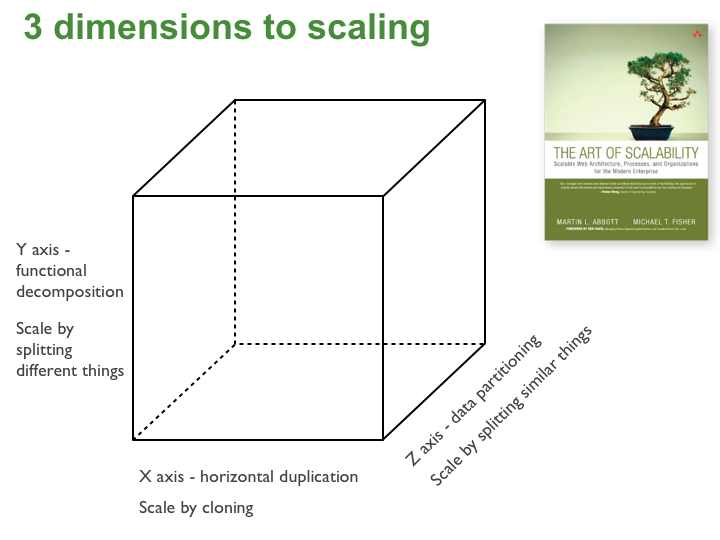
\includegraphics{img/ScaleCude.jpg}
\caption{Scaling Cube\citep{scale-cube}\label{scalecube}}
\end{figure}

Ahogy a \ref{scalecube}. ábrán is látható a meghatározó felbontási
fogalmak, az adat menti felbontás, a tetszőleges fogalom menti
felbontás, illetve a klónozás.

\subsubsection{Adat menti felbontás}\label{adat-menti-felbontuxe1s}

Az adat menti felbontás annyit tesz, hogy a szolgáltatásokat annak
megfelelően bontjuk fel, hogy milyen erőforrással dolgoznak, vagy
konkrétan egy adattal kapcsolatos összes funkciót egy helyen készítünk
el.

Példa: Erőforrás szerinti felbontás ha külön található szolgáltatás,
amivel az adatbázis műveleteket hajtjuk végre, és külön van olyan is,
ami csak a HTTP kéréseket szolgálja ki. Az egy adatra épülő módszernél
pedig alapul vehetünk egy olyan példát, ahol mondjuk egy szolgáltatás az
összes adminisztrátori funkciót látja el, míg más szolgáltatások a
más-más kategóriába eső felhasználók műveleteit hajtják végre.

Mivel a mikroszolgáltatások elve a hardvert is megosztja nem csak a
szoftvert, ezért az erőforrás szerinti szétválasztás kissé
értelmetlennek tűnhet, azonban a különböző platformok különböző
erőforrásait megéri külön szolgáltatásként kezelni. Ha egy
mikroszolgáltatást tartunk arra, hogy az adatbázis kéréseket
kiszolgálja, akkor az adatbázis nem oszlik meg a szolgáltatások között.
Ennek ellenére pazarló lehet minden szolgáltatásnak saját adatbázist
fenntartani.

\subsubsection{Fogalmi felbontás}\label{fogalmi-felbontuxe1s}

A tetszőleges fogalom menti felbontás annyit tesz hogy elosztott
rendszert hozunk létre tetszőleges funkcionalitás szerint. Erre épít a
mikroszolgáltatás architektúra is, mivel a lényege pont az egyes
funkciók atomi felbontása.

Példa: Adott egy könyvtár nyilvántartó rendszere, és ezt akarjuk
fogalmanként szétvágni. Külön-külön lehet szolgáltatást csinálni a
keresésnek, indexelésnek, foglalásnak, kivett könyvek nyilvántartásának,
böngészésre, könyvek adatainak tárolására, kiolvasására, és ehhez
hasonló funkciókra. Ezekkel a szétválasztásokkal a könyvtár működését
kis részekre bontottuk, és egy-egy kis szolgáltatásként könnyen
elérhetők.

\subsubsection{Klónozás}\label{kluxf3nozuxe1s}

A harmadik módszer arra tér ki, hogy hogyan lehet egy architektúrát
felosztani, hogy skálázható legyen. Itt a klónozhatóság, avagy az egymás
melletti kiszolgálás motivál. Ez a mikroszolgáltatásoknál kell, hogy
teljesüljön, mivel adott esetben egy terheléselosztó alatt tudnunk kell
definiálni több példányt is egy szolgáltatásból. Azért szükséges a
skálázhatóság a mikroszolgáltatások esetén, mivel kevés hardver mellett
is hatékonyan kialakítható az architektúra, de könnyen lehet szűk
keresztmetszetet létrehozni, amit skálázással könnyen megkerülhetünk.

\subsection{Architektúrális mintákhoz való
viszonya}\label{architektuxfaruxe1lis-mintuxe1khoz-valuxf3-viszonya}

Mint korábban láthattuk vannak bizonyos telepítési módszerek, amik
mentén szokás a mikroszolgáltatásokat felépíteni. Van aki az
architektúrális tervezési minták közé sorolja a mikroszolgáltatás
architektúrát, de nem könnyű meghatározni, hogy hogyan is alkot önálló
mintát. Nagyon sok lehetőség van a mikroszolgáltatásokban, és leginkább
más architektúrákkal együtt használva lehet hatékonyan és jól használni.

Nézzünk meg három felhasználható architektúrális mintát:

\subsubsection{Pipes and Filters}\label{pipes-and-filters}

A Pipes and filter architektúrális minta\citep{pipes-pattern} lényege,
hogy a funkciókra bontott architektúrát az elérni kívánt végeredmény
érdekében különböző módokon összekötjük. Ebben a módszerben az adat
folyamatosan áramlik az egyes alkotó elemek között, és lépésről lépésre
alakul ki a végeredmény. Elég olcsón kivitelezhető architektúrális
minta, mivel csupán sorba kell kötni hozzá az egyes szolgáltatásokat,
azonban nehezen lehet optimalizálni, és könnyen lehet, hogy olyan részek
lesznek a feldolgozás közben, amik hátráltatják a teljes folyamatot.

\subsubsection{Publisher/Subscriber}\label{publishersubscriber}

Egy másik, elosztott rendszerekhez kitalált minta a
publisher/subscriber\citep{pub-subscribed}, amely azon alapszik, hogy
egy szolgáltatásnak szüksége van valamilyen adatra vagy funkcióra, és
ezért feliratkozik egy másik szolgáltatásra. Ennek az lesz az eredménye,
hogy bizonyos szolgáltatások, bizonyos más szolgáltatásokhoz fognak
kötődni, és annak megfelelően fognak egymással kommunikálni, hogy milyen
feladatot kell végrehajtaniuk.

\subsubsection{Esemény alapú
architektúra}\label{esemuxe9ny-alapuxfa-architektuxfara}

Az esemény alapú architektúrákat\citep{event-driven-pattern} könnyen
kialakíthatjuk, ha egy mikroszolgáltatásokból álló rendszerben olyan
alkalmazásokat és komponenseket fejlesztünk ahol eseményeken keresztül
kommunikálnak az egyes elemek. Ezzel a nézettel olyan struktúrát lehet
összeépíteni, ahol a kis egységek szükség szerint kommunikálnak, és a
kommunikáció egy jól definiált interfészen keresztül történik.

\subsection{Eltérések a szolgáltatás orientált
architektúrától}\label{eltuxe9ruxe9sek-a-szolguxe1ltatuxe1s-orientuxe1lt-architektuxfaruxe1tuxf3l}

A mikroszolgáltatások a szolgáltatás orientált architektúrális minta
finomítása, mivel elsősorban szeparált egységeket, önműködő
szolgáltatásokat hoz létre, amik életképesek önmagukban is, és amennyire
lehet oszthatatlanok. A szolgáltatás orientált esetben viszont a meglévő
szolgáltatásainkat kapcsoljuk össze, ami akár egy helyen is futhat és
egyáltalán nem az atomicitás a lényege.

\subsection{Példák mikroszolgáltatásokat használó
alkalmazásokra}\label{puxe9lduxe1k-mikroszolguxe1ltatuxe1sokat-hasznuxe1luxf3-alkalmazuxe1sokra}

Ugyan a mikroszolgáltatásokra épülő architektúra egy viszonylag új
fejlesztési módszer, de találhatunk az iparban erre épülő
alkalmazásokat. Az alábbi vállalatok átalakították, vagy elkeztdék
átalakítani a szolgáltatásaikat ennek a módszernek megfelelően:

\begin{itemize}
\item
  \textbf{Amazon}: Az Amazon Cloud szolgáltatása, és web áruháza is
  szolgáltatásokká átalakította, mivel a legtöbb funkció amit a
  felhasználók elérhetnek, interaktívan kommunikálnak, és minden
  feladathoz tartozó implementáció külön szolgáltatásokra van szedve.
  Ugyan vannak összetett funkciók mint a skálázás, ami több funkció
  együttesétől függ, de a háttérben a szolgáltatások közötti
  kommunikáció zajlik. (vm monitoring, vm create, vm start, stb.)
\item
  \textbf{eBay}: Az eBay vásárló oldala kezdetektől fogva
  szolgáltatásokra volt bontva, de elkezdték szétbontani kisebb alkotó
  elemekre őket, illetve saját konténerekben futtatják a funkciókat.
  Elkülönített szolgáltatásként szerepel például a vásárlás, vagy a
  megrendeléshez tartozó szolgáltatás.
\item
  \textbf{NetFlix}: A NetFlix videomegosztó alkalmazása, az eBay-hez
  hasonlóan szolgáltatásokra volt bontva, azonban a streaming álltal
  okozott skálázási problémák miatt elkezdték átalakítani a
  részegységeket a mikroszolgáltatások elve szerint.
\item
  \textbf{Archivematica}: Az Archivematica\citep{archivematica} egy
  nyílt forráskódú elektronikus tartalom kezelő, ami tud kezelni
  különböző fájlokat, multimédiás adatokat, illetve akármilyen szöveges
  tartalmat. Ez az alkalmazás alapvetően monolitikus architektúrára
  épül, azonban elkezdték átalakítani a struktúráját
  mikroszolgáltatásokat használó architektúrára. Ezt úgy kivitelezték,
  hogy a különböző plusz funkciókat az eredeti alkalmazás plugin-szerűen
  mikroszolgáltatásokból nyeri ki, és ennek megfelelően a tovább
  fejlesztés is megalapozott\citep{archivematica-wiki}.
\end{itemize}

\section{Mikroszolgáltatások előnyei és
hátrányai}\label{mikroszolguxe1ltatuxe1sok-elux151nyei-uxe9s-huxe1truxe1nyai}

Ahogy minden architektúrális mintának, a mikroszolgáltatásoknak is
vannak előnyei\citep{microservices}, amik indokolttá teszik a minta
használatát, és vannak hátrányai\citep{micro-disadv}, amiket
mérlegelnünk kell a tervezés folyamán.

\subsection{Előnyök}\label{elux151nyuxf6k}

\subsubsection{Könnyű fejleszteni}\label{kuxf6nnyux171-fejleszteni}

Mivel kis részekre van szedve az alkalmazásunk, a fejlesztést akár több
csapatnak is ki lehet osztani, hogy az alkalmazás részeit alkossák meg,
hiszen önállóan is életképesek a szolgáltatások. Az egyes szolgáltatások
nem rendelkeznek túl sok logikával, így kis méretű könnyen kezelhető
feladatokkal kell a csapatoknak foglalkozni.

\subsubsection{Egyszerűen
megérthető}\label{egyszerux171en-meguxe9rthetux151}

Egy szolgáltatás nagyon kis egysége a teljes alkalmazásnak, így könnyen
megérthető. Kevés technológia, és kevés kód áll rendelkezésre egy
szolgáltatásnál, így gyorsan beletanulhat egy új fejlesztő a munkába. A
dokumentáció, átláthatóság, illetve a hibák analizálása közben is jól
jön, hogy élesen elvállnak az egyes egységek.

\subsubsection{Könnyen kicserélhető, módosítható,
telepíthető}\label{kuxf6nnyen-kicseruxe9lhetux151-muxf3dosuxedthatuxf3-telepuxedthetux151}

A szolgáltatások önállóan is működnek, így az azonos interfésszel
rendelkező szolgáltatásra bármikor kicserélhető, illetve módosítható ha
megmaradnak a korábbi funkciók. A szolgáltatás telepítése is egyszerű,
mivel csak kevés környezeti feltétele van annak, hogy egy ilyen kis
méretű program működni tudjon. A fejlesztést nagyban segíti, hogy egy
korábbi verziójú alkalmazásba plugin-szerűen be lehet integrálni az
újonnan fejlesztett részeket, mivel ez gyors visszajelzést ad a
fejlesztőknek. Ez a tulajdonsága a folytonos integrációt támogató
eszközöknél is előnyös, mivel könnyen lehet vele automatizált
metodológiákat készíteni.

\subsubsection{Jól skálázható}\label{juxf3l-skuxe1luxe1zhatuxf3}

Mivel sok kis részletből áll az alkalmazásunk, nem szükséges minden
funkciónkhoz növelni az erőforrások allokációját, hanem kis
komponensekhez is lehet rendelni több erőforrást. Például egy számítási
felhőben, a teljesítményben látható változásokat könnyen és gyorsan
lehet kezelni, a problémát okozó funkció felskálázásával.

\subsubsection{Támogatja a kevert
technológiákat}\label{tuxe1mogatja-a-kevert-technoluxf3giuxe1kat}

Az egyik legnagyobb ereje ennek az architektúrának, hogy képes egy
alkalmazáson belül kevert technológiákat is használni. Mivel egy jól
definiált interfészen keresztül kommunikálnak a szolgáltatások, ezért
mindegy milyen technológia van mögötte, amíg ki tudja szolgálni a
feladatát. Ennek megfelelően el tudunk helyezni egy Linux-os
környezetben használt LDAP-ot, és egy Windows-os környezetben használt
Active Directory-t is, és minden gond nélkül használni is tudjuk őket az
interfésziek segítségével.

\subsection{Hátrányok}\label{huxe1truxe1nyok}

\subsubsection{Komplex alkalmazás alakul
ki}\label{komplex-alkalmazuxe1s-alakul-ki}

Mivel minden funkcióra saját szolgáltatást csinálunk, nagyon sok lesz az
elkülönülő elem, és a teljes alkalmazás egyben tartása nagyon nehéz
feladattá válik. Mivel fontos a szolgáltatások együttműködése, a sok
interfésznek ismernie kell egymást, és fenn kell tartani a
konzisztenciát minden szolgáltatással.

\subsubsection{Nehezen kezelhető az elosztott
rendszer}\label{nehezen-kezelhetux151-az-elosztott-rendszer}

A mikroszolgáltatások architektúra egy elosztott rendszert ír le, és
mint minden elosztott rendszer ez is bonyolultabb lesz a monolitikus
változatánál. Elosztott rendszereknél figyelni kell az adatok
konzisztenciáját, a kommunikáció plusz feladatot ad minden szolgáltatás
fejlesztőjének, és folyamatosan együtt kell működni a többi szolgáltatás
fejlesztőjével.

\subsubsection{Plusz munkát jelenthet az aszinkron üzenet
fogadás}\label{plusz-munkuxe1t-jelenthet-az-aszinkron-uxfczenet-fogaduxe1s}

Mivel egy szolgáltatás egyszerre több kérést is ki kell hogy szolgáljon
egyszerűbb ha aszinkron módon működik. Ezt azonban mindig le kell
implementálni, és az aszinkron üzenetek bonyolítják az adatok kezelését.
Az egyes szolgáltatások között könnyen lehetnek adatbázisbeli
inkonzisztenciák, mivel aszinkron működés esetén nem minden kiszolgált
kérésnek ugyan az a ritmusa. Ugyan nem megoldhatatlan feladat ezeket az
időbeli problémákat lekezelni, de plusz komplexitást hozhat be, amit egy
közös környezetben lock-olással könnyedén megoldhatnánk.

\subsubsection{Kód duplikátumok
kialakulása}\label{kuxf3d-duplikuxe1tumok-kialakuluxe1sa}

Amikor nagyon hasonló (kis részletben eltérő) szolgáltatásokat
csinálunk, megesik, hogy ugyan azt a kódot többször fel kell
használnunk, és ezzel kód, és adat duplikátumok keletkeznek, amiket le
kell kezelnünk. Nem nehéz találni olyan példát, ahol a létrehozás és
szerkesztés művelete megvalósítható ugyan külön szolgáltatásként,
viszont nehezíti a feladatot, hogy 2 külön adatbázist kéne módosítani az
ideális megvalósításban, és ezek konzisztenciáját fenn kéne tartani.

\subsubsection{Interfészek
fixálódnak}\label{interfuxe9szek-fixuxe1luxf3dnak}

A fejlesztés folyamán a szolgáltatásokhoz rendelt interfészek
fixálódnak, és ha módosítani akarunk rajta, akkor több szolgáltatásban
is meg kell változtatni az interfészt. Ennek a problémának a megoldása,
alapos tervezés, és sokszintű, bonyolult interfész struktúra
használatával megoldható.

\subsubsection{Nehezen tesztelhető
egészben}\label{nehezen-tesztelhetux151-eguxe9szben}

Mivel sok kis részletből rakódik össze a nagy egész alkalmazás, a
tesztelési fázisban kell olyan teszteket is végezni, ami a rendszer
egészét, és a kész alkalmazást teszteli. Egy ilyen teszt elkészítése
bonyolult lehet, és plusz feladatot ad a sok szolgáltatás külön-külön
fordítása, és telepítése is.

\subsection{Összehasonlítva a monolitikus
architektúrával}\label{uxf6sszehasonluxedtva-a-monolitikus-architektuxfaruxe1val}

A mikroszolgáltatás architektúra és a monolitikus architektúra egymás
ellentettjei, melyben az erőforrások központilag vannak kezelve, és
minden funkció egy nagy interfészen keresztül érhető el. A monolitikus
architektúra egyszerűen kiépíthető, könnyű tervezni és fejleszteni,
azonban nehezen lehet kicserélni, nem elég robosztus, és nehezen
skálázható, mivel az erőforrásokat közösen kezelik a funkciók.

Ezzel ellentétben a mikroszolgáltatás architektúrát nehezen lehet
megtervezni, hiszen egy elosztott rendszert kell megtervezni, ahol az
adatátviteltől kezdve az erőforrás megosztáson keresztül semmi sem
egyértelmű. A kezdeti nehézségek után viszont a későbbi továbbfejlesztés
sokkal egyszerűbb, mivel külön csapatokat lehet rendelni az egyes
szolgáltatásokhoz, és könnyen integrálhatók, kicserélhetők az alkotó
elemek. Mivel sok kis egységből áll, könnyebben lehet úgy skálázni a
rendszert, hogy ne pazaroljuk el az erőforrásainkat, és ugyanakkor a kis
szolgáltatások erőforrásokban is el vannak különítve, így nem okoz
gondot, hogy fel vagy le skálázzunk egy szolgáltatást. Ennek az a
hátránya, hogy le kell kezelni a skálázáskor a közös
erőforrásokat.(Például ha veszünk egy autentikációs szolgáltatást, akkor
ha azt fel skálázzuk, meg kell tartanunk a felhasználók listáját, így
duplikálni kell az adatbázist, és fenntartani a konzisztenciát) Ugyan
csak előnye a mikroszolgáltatás architektúrának, hogy különböző
technológiákat lehet keverni vele, mivel az egyes szolgáltatások
különböző technológiákkal különböző platformon is futhatnak.

\section{Technológiai
áttekintés}\label{technoluxf3giai-uxe1ttekintuxe9s}

Az integrációhoz olyan technológiákat\citep{micro-introPt1} lehet
használni, melyek lehetővé teszik az egyes szolgáltatások elkülönült
működését. Ahhoz, hogy jó technológiákat válasszunk, mindeképpen
ismernünk kell az igényeket, mivel a technológiák széles köre áll
rendelkezésünkre. Fontos szem előtt tartani pár általános érvényű
szabályt is\citep{micro-golden}, ami a mikroszolgáltatások helyes
működéséhez kell. Ezek pedig a következők:

\begin{itemize}
\tightlist
\item
  Modulárisan szétválasztani a szolgáltatásokat
\item
  Legyenek egymástól teljesen elkülönítve
\item
  Legyen jól definiált a szolgáltatások kapcsolata
\end{itemize}

A következő feladatokra kellenek technológiák:

\begin{itemize}
\tightlist
\item
  Hogyan lehet feltelepíteni egy önálló szolgáltatást? (telepítés,
  folytonos integráció)
\item
  Hogyan lehet összekötni ezeket a szolgáltatásokat? (automatikus
  környezet felderítés)
\item
  Hogyan lehet fenntartani, változtatni a szolgáltatások környezetét?
  (konfiguráció menedzsment)
\item
  Hogyan lehet skálázni a szolgáltatást? (skálázás)
\item
  Hogyan lehet egységesen használni a skálázott szolgáltatásokat? (load
  balance, konzisztencia fenntartás)
\item
  Hogyan lehet virtualizáltan ezt kivitelezni? (virtualizálás)
\item
  A meglévő szolgáltatásokat hogyan tartsuk nyilván? (szolgáltatás
  jegyzék)
\item
  Hogyan figyeljük meg az alkalmazást működés közben (monitorozás,
  loggolás)
\end{itemize}

\subsection{Futtatókörnyezetek}\label{futtatuxf3kuxf6rnyezetek}

A mikroszolgáltatásokat valamilyen módon létre kell hozni, egy hosthoz
kell rendelni, és az egyes elemeket össze kell kötni. A szolgáltatások
telepítéséhez olyan technológiára van szükség amivel könnyen elérhetünk
egy távoli gépet, és könnyen kezelhetjük az ottani erőforrásokat. Ehhez
a legkézenfekvőbb megoldás a Linux rendszerek esetén az SSH kapcsolaton
keresztül végrehajtott Bash parancs, de vannak eszközök, amikkel ezt
egyszerűbben és elosztottabban is megtehetjük.

\begin{itemize}
\item
  \textbf{ElasticBox}\citep{elasticbox}: Egy olyan alkalmazás, melyben
  nyilvántarthatjuk az alkalmazásainkat, és könnyen egyszerűen
  telepíthetjük őket. Támogatja a konfigurációk változását, illetve
  számos technológiát, amivel karbantarthatjuk a környezetünket (Docker,
  Puppet, Ansible, Chef, stb). Együtt működik különböző számítási felhő
  megoldásokkal, mint az AWS, vSphere, Azure, és más környezetek.
  Mindent végre tud hajtani ami egy mikroszolgáltatás alapú
  alkalmazáshoz szükséges, teljes körű felügyeletet biztosít.
  \citep{jenkins-elasticbox}
\item
  \textbf{Kubernetes}\citep{kubernetes}: A Kubernetes az ElasticBox egy
  opensource változata, ami lényegesen kevesebbet tud, azonban
  ingyenesen elérhető. Ez a projekt még nagyon gyerekcipőben jár, így
  nem tudom felhasználni a félév során.
\end{itemize}

Egyéb lehetőség, hogy a fejlesztő készít magának egy olyan szkriptet,
ami elkészíti számára a mikroszolgáltatás alapú architektúrát, és
lehetővé teszi az elemek dinamikus kicserélését (ad-hoc megoldás). Ennek
a megoldásnak a hátránya hogy nincs támogatva, és minden funkciót külön
kell implementálni. Sokkal nagyobb erőforrásokat emészthet fel mint egy
ingyenes, vagy nyílt forrású megoldást választani.

\subsection{Folytonos Integrációt támogató
eszközök}\label{folytonos-integruxe1ciuxf3t-tuxe1mogatuxf3-eszkuxf6zuxf6k}

Mivel az mikroszolgáltatások fejlesztését, tesztelését, és minden
funkcióját, eszközét figyelnünk kell, ezért nem árt, ha van egy
folytonos integrációt támogató keretrendszer, ami képes figyelni a
mikroszolgáltatásokhoz tartozó eszközöket, segíti a fejlesztés
folyamatát azzal, hogy automatizáltan végrehajtja a szolgáltatások
fordítását, telepítését, és tesztelését. Ezek az eszközök leginkább a
fejlesztés folyamtában használhatók fel, de van olyan belőlük, amivel
tetszőlegesen komplex feladatokat is végrehajthatunk az
alkalmazásunkkal.

\begin{itemize}
\item
  \textbf{Jenkins}\citep{jenkins}: A Jenkins egy olyan folytonos
  integráláshoz kifejlesztett eszköz, mellyel képesek vagyunk különböző
  funkciókat automatizálni, vagy időzítetten futtatni. A Jenkins egy
  Java alapú webes felülettel rendelkező alkalmazás, amely képes Bash
  parancsokat futtatni, Docker konténereket kezelni, build-eket
  futtatni, illetve a hozzá fejlesztett plugin-eken keresztül, szinte
  bármire képes. Támogatja a fürtözést is, így képesek vagyunk Jenkins
  slave-eket létrehozni, amik a mester szerverrel kommunikálva végzik el
  a dolgukat. A mikroszolgáltatás architektúrák esetén alkalmas minden
  feladatot ellátni, és véghez vinni a fordítást, telepítést, és
  tesztelést.
\item
  \textbf{Travis CI}\citep{travis}: A Travis CI egy olyan Cloud
  szolgáltatás, amely képes teszteket, és fordítást végezni egy megadott
  Github projektből, és ehhez egy teljesen tiszta virtuális környezetet
  használ fel. A rendszer a saját beépített támogató moduljain keresztül
  képes kiszolgálni a felhasználó kéréseit, amit a Jenkins-hez hasonló
  módon tesz. A Jenkins-hez képest nincs teljes kontrollunk a teljes
  architektúra felett, nem támogat bármely verziókezelőt, és
  mikroszolgáltatások esetén a szolgáltatás konténerének a meghatározása
  is nehézségekbe ütközik, azonban a kezdeti egység tesztelésre, és
  funkció tesztek futtatására alkalmas.
\end{itemize}

Folytonos integrációt támogató keretrendszert sok erőfeszítés lenne
kézileg elkészíteni, mivel összetett kapcsolatokat kell kiépítenie a
végrehajtandó folyamatok közben, aminek az implementálása nem triviális,
és egy ingyenesen használható eszköz sokkal könnyebben
felkonfigurálható.

\subsection{Környezet felderítési
technológiák}\label{kuxf6rnyezet-felderuxedtuxe9si-technoluxf3giuxe1k}

Az egyes szolgáltatásoknak meg kell találniuk egymást, hogy megfelelően
működhessen a rendszer, azonban ez nem mindig triviális, így szükség van
egy olyan alkalmazásra, amivel felderíthetjük az aktív szolgáltatásokat.

\begin{itemize}
\item
  \textbf{Consul}\citep{consul}: A Hashicorp szolgáltatásfelderítő
  alkalmazása, amely egy kliens-szerver architektúrának megfelelően
  megtalálja a környezetében lévő szolgáltatásokat, és figyeli az
  állapotukat (ha inaktívvá válik egy szolgáltatás a Consul észre
  veszi). Ez az alkalmazás egy folyamatosan választott mester állomásból
  és a többi slave állomásból áll. A mester figyeli az alárendelteket,
  és kezeli a kommunikációt. Egy új slave-et úgy tudunk felvenni, hogy a
  consul klienssel kapcsolódunk a mesterre. Ha automatizáltan tudjuk
  vezényelni a feliratkozást, egy nagyon erős eszköz kerül a kezünkbe,
  mivel eseményeket küldhetünk a szervereknek, és ezekre különböző
  feladatokat hajthatunk végre.
\item
  \textbf{Serf}\citep{serf}: A Hashicorp egy másik hálózati felderítő
  eszköze, ami elosztottan nagy rendelkezésre állással képes a fürtözött
  elemek között fenntartani a kapcsolatot. Ugyan elsősorban fürtözött
  elemek közé tervezték, de tetszőleges kapcsolat felderítésre, és
  nyilvántartására alkalmas. A Consul-hoz hasonló módon egy saját
  protokollon keresztül kommunikál a többi serf ágenssel, de nem
  szükséges neki szerver-kliens kapcsolat. Képes egyszerű események
  küldésére, azonban a szolgáltatásokat nem képes külön kezelni, inkább
  csak a végpont állapotát figyeli.
\end{itemize}

A kézi megoldás itt is lehetséges, mivel saját névfeloldás esetén a
névfeloldó szervert használhatjuk az egyes állomások felderítésére, vagy
Docker-t használva a Docker hálózatok elérhetővé teszik a
szolgáltatásokat a futtató konténer hoszt nevével.

\subsection{Konfiguráció
menedzsment}\label{konfiguruxe1ciuxf3-menedzsment}

A telepítéshez és a rendszer állapotának a fenntartásához egy olyan
eszköz kell, amivel gyorsan egyszerűen végrehajthatjuk a
változtatásainkat, és minden újdonság az összes egyforma komponensen be
lesz állítva.

\begin{itemize}
\item
  \textbf{Puppet}\citep{puppet}: Olyan nyílt forrású megoldás, amellyel
  leírhatjuk objektum orientáltan, hogy milyen változtatásokat akarunk
  elérni, és a Puppet elvégzi a változtatásokat. Automatizálja a
  szolgáltatás változtatásának minden lépését, és egyszerű, gyors
  megoldást szolgáltathat a komplex rendszerbe integráláshoz.
\item
  \textbf{Chef}\citep{chef}: A Chef egy olyan konfiguráció menedzsment
  eszköz ami nagy mennyiségű szerver számítógépet képes kezelni,
  fürtözhető, és megfigyeli az alá szervezett szerverek állapotát.
  Tartja a kapcsolatot a gépekkel, és ha valamelyik konfiguráció nem
  felel meg a definiált receptkönynek, (amiben definiálhatjuk az elvárt
  környezeti paramétereket) akkor változtatásokat indít be, és eléri,
  hogy a szerver a megfelelő konfigurációval rendelkezzen. Népszerű
  konfiguráció menedzsment eszköz, amit könnyedén használhatunk
  integrációhoz, illetve a szolgáltatások cseréjéhez, és
  karbantartásához.
\item
  \textbf{Ansible}\citep{ansible}: A Chef-hez hasonlóan képes
  változtatásokat eszközölni a szerver gépeken egy ágens nélküli SSH
  kapcsolaton keresztül, viszont a Chef-el ellentétben nem tartja a
  folyamatos kapcsolatot. Az Ansible egy tipikusan integrációs célokra
  kifejlesztett eszköz, amelyhez felvehetjük a gépeket, amiken
  valamilyen konfigurációs változtatást akarunk végezni, és egy
  ``playbook'' segítségével leírhatjuk milyen változásokat kell
  végrehajtani melyik szerverre. Könnyen irányíthatjuk vele a
  szolgáltatásokat, és definiálhatunk szolgáltatásonként egy playbook-ot
  ami mondjuk egy fürtnyi szolgáltatást vezérel. Ez az eszköz hasznos
  lehet, ha egy szolgáltatásnak elő akarjuk készíteni a környezetet.
\item
  \textbf{SaltStack}\citep{saltstack}: A SaltStack nagyon hasonlít a
  Chef-re, mivel ez a termék is széleskörű felügyeletet, és konfiguráció
  menedzsmentet kínál számunkra, amit folyamatos kapcsolat
  fenntartással, és gyors kommunikációval ér el. Az Ansible-höz nagyon
  hasonlóan konfigurálható, szintén ágens nélküli kapcsolatot tud
  létesíteni, és a Chef-hez hasonlóan több 10 ezer gépet tud egyszerre
  karbantartani.
\end{itemize}

Minden konfigurációs menedzsment eszköznek megvan a saját nyelve, amivel
deklaratívan le lehet írni, hogy mit szeretnénk változtatni, és azokat a
program beállítja. Erre a feladatra nem nagyon érdemes saját eszközt
készíteni, mivel számos megoldás elérhető, és a megvalósítás komoly
tervezést, és fejlesztést igényel. Érdemes megemlíteni a Docker
konténerek adta lehetőséget, mivel a Docker konténerek gyorsan
konfigurálhatók, fejleszthetők, és a konténer képeken keresztül jól
karbantarthatók, így a konfiguráció menedzsment is megoldható velük. Ami
hiányzik ebből a megoldásból az a többi szolgáltatás értesítése a
változtatásról.

\subsection{Terheléselosztás}\label{terheluxe9selosztuxe1s}

A mikroszolgáltatás alapú architektúrának egyik fontos eleme a
terheléselosztó, vagy valamilyen fürtözést lehetővé tevő eszköz. Ez
azért fontos, mert egy egységes interfészt tudunk kialakítani a
szolgáltatásaink elérésére, és könnyíti a skálázódást a szolgáltatások
mentén.

\begin{itemize}
\item
  \textbf{HAProxy}\citep{haproxy} \citep{LB-haproxy}: Egy magas
  rendelkezésre állást biztosító, és megbízhatóságot növelő
  terheléselosztó eszköz. Konfigurációs fájlokon keresztül
  megszervezhetjük, hogy mely gépet hogyan érjünk el, milyen IP címek
  mely szolgáltatásokhoz tartoznak, illetve választhatóan round robin,
  legkisebb terhelés, session alapú, vagy egyéb módon osztja szét a
  kéréseket az egyes szerverek között. Ez az eszköz csak és kizárólag a
  HTTP TCP kéréseket tudja elosztani, de egyszerű, könnyen telepíthető,
  és könnyen kezelhető (ha nem dinamikusan változnak a fürtben lévő
  gépek, mert ha igen akkor szükséges egy mellékes frissítő logika is).
\item
  \textbf{Ngnix}\citep{nginx}: Az Nginx egy nyílt forráskódú web
  kiszolgáló és reverse proxy szerver, amivel nagy méretű rendszereket
  kezelhetünk, és segít az alkalmazás biztonságának megőrzésében. A
  kiterjesztett változatával (Nginx Plus) képesek lehetünk a
  terheléselosztásra, és alkalmazás telepítésre. Nem teljesen a proxy
  szerver szerepét váltja ki, de képes elvégezni azt.
\end{itemize}

A kézi megvalósítás gyakorlatilag egy kézileg implementált
terheléselosztó eszköz lenne, amihez viszont hálózati megfigyelés, és
routing szükséges, így nem javallott ilyen eszköz készítése.

\subsection{Skálázási
technológiák}\label{skuxe1luxe1zuxe1si-technoluxf3giuxe1k}

A mikroszolgáltatás alapú architektúrák egyik nagy előnye, hogy az egyes
funkciókra épülő szolgáltatásokat könnyedén lehet skálázni, mivel egy
terheléselosztót használva csupán egy újabb gépet kell beszervezni, és
máris nagyobb terhelést is elbír a rendszer. Ahhoz hogy ezt kivitelezni
tudjuk, szükségünk van egy terheléselosztóra, és egy olyan logikára, ami
képes megsokszorozni az erőforrásainkat. Számítási felhő alapú
környezetben ez könnyen kivitelezhető, egyébként hideg tartalékban
tartott gépek behozatalával elérhető. Sajnálatos módon általános célú
skálázó eszköz nincsen a piacon, viszont gyakran készítenek maguknak
saját logikát a nagyobb gyártók.

\begin{itemize}
\item
  \textbf{Elastic Load Balancer}\citep{elastic-load-balance}: Az Amazon
  AWS-ben az ELB avagy rugalmas terheléselosztó az, ami ezt a célt
  szolgálja. Ennek a szolgáltatásnak az lenne a lényege, hogy segítse az
  Amazon Cloud-ban futó virtuális gépek hibatűrését, illetve egységbe
  szervezi a különböző elérhetőségi zónákban lévő gépeket, amivel
  gyorsabb elérést tudunk elérni. Mivel ez a szolgáltatás csupán az
  Amazon AWS-t felhasználva tud működni, nem megfelelő általános célra,
  azonban ha az Amazon Cloud-ban építjük fel a mikroszolgáltatás alapú
  architektúránkat, akkor erős eszköz lehet számunkra.
\item
  \textbf{Terheléselosztó használata}: Vannak olyan terheléselosztók,
  melyek bizonyos szolgáltatásokat nyújtó gépeket képesek automatikusan
  skálázni. Ilyen a HAProxy, és az Ngnix is. Például a HAProxy a TCP
  üzeneteket képes fogadni és elosztani a hozzá beregisztrált gépek
  között, és beállítástól függően képes kezelni automatikusan gépeket
  elvenni, vagy hozzáadni a hálózathoz.
\end{itemize}

A skálázás egyik legegyszerűbb megvalósítása, hogy egy proxy szervert
felhasználva, valamilyen módon egységesen elosztjuk a kéréseket, és egy
saját monitorozó eszközzel figyeljük a terhelést (processzor terheltség,
memória, hálózati terhelés). Ha valamelyik érték megnő, egy ágenses vagy
ágens nélküli technológiával a virtualizált környezetben egy új példányt
készítünk a terhelt szolgáltatásból, és a proxy automatikusan megoldja a
többit. Nem tökéletes megoldást kapunk, azonban ez a legtöbb
felhasználási esetben megfelelőnek bizonyul.

\subsection{Virtualizációs
technológiák}\label{virtualizuxe1ciuxf3s-technoluxf3giuxe1k}

A mikroszolgáltatás alapú architektúrák kialakításánál nagy előnyt
jelenthet, ha valamilyen virtualizációt használunk fel a környezet
kialakításához. Virtualizált környezetben könnyebb a telepítés,
skálázás, és a monitorozás is.

\begin{itemize}
\item
  \textbf{Docker}\citep{docker}: Egy konténer virtualizációs eszköz,
  amelynek segítségével egy adott kernel alatt több különböző
  környezettel rendelkező, alkalmazásokat futtató környezetet hozhatunk
  létre. A Docker egy szeparált fájlrendszert hoz létre a gazda gépen,
  és abban hajt végre műveleteket. Készíthetünk vele előre elkészített
  alkalmazás környezeteket, és szolgáltatásokat, ami ideálissá teszi
  mikroszolgáltatás alapú architektúrák létrehozásánál. A Docker
  konténerek segítségével egyszerűen telepíthetjük, skálázhatjuk, és
  fejleszthetjük a rendszert.
\item
  \textbf{libvirt}\citep{libvirt}: Többféle virtualizációs
  technológiával együtt működő eszköz, amivel könnyedén irányíthatjuk a
  virtuális gépeket, és a virtualizálás komolyabb részét el
  absztrahálja. Támogat KVM-em, XEN-t, VirtualBox-ot, LXC-t, és sok más
  virtualizáló technológiát. Ezzel az eszközzel a környezet kialakítását
  szabhatjuk meg, tehát a hardveres erőforrások megosztásában nyújt nagy
  segítséget.
\item
  \textbf{KVM}\citep{kvm}: A KVM egy kernel szintű virtualizációs
  eszköz, amivel virtuális gépeket tudunk készíteni. Processzor szintjén
  képes szétválasztani az erőforrásokat, és ezzel szeparált
  környezeteket létrehozni. Virtualizál a processzoron kívül hálózati
  kártyát, háttértárat, grafikus meghajtót, és sok mást. A KVM egy nyílt
  forráskódú projekt és létrehozhatunk vele Linux és Windows gépeket is
  egyaránt.
\item
  \textbf{Kereskedelmi cloud szolgáltatás}: Ha virtualizációról
  beszélünk, akkor adja magát hogy a számítási felhőket is ide értsük.
  Egy mikroszolgáltatás architektúrájú programot a legcélszerűbb
  valamilyen számítási felhőben létrehozni, mivel egy ilyen környezetnek
  definíciója szerint tartalmaznia kell egy virtualizációs szintet,
  megosztott erőforrásokat, monitorozást, és egyfajta leltárat a futó
  példányokról. Ennek megfelelően a mikroszolgáltatás alapú architektúra
  minden környezeti feltételét lefedi, csupán a szolgáltatásokat,
  business logikát, és az interfészeket kell elkészítenünk. Jellemzően a
  Cloud-os környezetek tartalmaznak terheléselosztást, és skálázási
  megoldást is, amivel szintén erősítik a szolgáltatás alapú
  architektúrákat. Ilyen környezet lehet az Amazon, Microsoft Azure,
  Google App Engine, OpenStack, és sokan mások.
\end{itemize}

Amennyiben nincs a kezünkben egy saját virtualizáló eszköz, a
virtualizálás kézi megvalósítása értelmetlen plusz komplexitást ad az
alkalmazáshoz.

\subsection{Szolgáltatás jegyzékek (service
registry)}\label{szolguxe1ltatuxe1s-jegyzuxe9kek-service-registry}

Számon kell tartani, hogy milyen szolgáltatások elérhetők, milyen címen
és hány példányban az architektúránkban, és ehhez valamilyen
szolgáltatás nyilvántartási eszközt\citep{service-registry-pattern}
\citep{micro-introPt3} kell használnunk.

\begin{itemize}
\item
  \textbf{Eureka}\citep{eureka-glance}: Az Eureka a Netflix fejlesztése,
  egy AWS környezetben működő terheléselosztó alkalmazás, ami figyeli a
  felvett szolgáltatásokat, és így mint nyilvántartás is megfelelő. A
  kommunikációt és a kapcsolatot egy Java nyelven írt szerver és kliens
  biztosítja, ami a teljes logikát megvalósítja. Együtt működik a
  Netflix álltal fejlesztett Asgard nevezetű alkalmazással, ami az AWS
  szolgáltatásokhoz való hozzáférést segíti. Ugyan ez az eszköz erősen
  optimalizált az Amazon Cloud szolgáltatásaihoz, de a leírás alapján
  megállja a helyét önállóan is. Mivel nyílt forráskódú, mintát
  szolgáltat egyéb alkalmazásoknak is.
\item
  \textbf{Consul}: Korábban már említettem ezt az eszközt, mivel abban
  segít, hogy felismerjék egymást a szolgáltatások. A kapcsolatot
  vizsgáló és felderítő logikán kívül tartalmaz egy nyilvántartást is a
  beregisztrált szolgáltatásokról, amiknek az állapotát is
  vizsgálhatjuk.
\item
  \textbf{Apache Zookeeper}\citep{zookeeper}: A Zookeeper egy
  központosított szolgáltatás, konfigurációs adatok és hálózati adatok
  karbantartására, ami támogatja az elosztott működést, és a szerverek
  csoportosítását. Ezt az eszközt elosztott alkalmazás fejlesztésre, és
  komplex rendszer felügyeletére és telepítés segítésére tervezték. A
  Consul-hoz hasonlóan működik, és a feladata is ugyan az.
\end{itemize}

Kézi megoldás erre nem nagyon van, csupán egy központi adatbázisban,
vagy leltár alkalmazásban elmentet adatokból tudunk valamilyen jegyzéket
csinálni, amihez viszont a szolgáltatások mindegyikének hozzá kell
férni. Könnyen konfigurálható megoldást kapunk, és tetszőleges adatot
menthetünk a szolgáltatásokról, de egyéb funkciók, mint az esemény
küldés és fogadás, csak bonyolult implementációval lehetséges.

\subsection{Monitorozás, loggolás}\label{monitorozuxe1s-loggoluxe1s}

Ha már megépítettük a mikroszolgáltatás alapú architektúrát, akkor meg
kell bizonyosodnunk róla, hogy minden megfelelően működik, és minden
rendben zajlik a szolgáltatásokkal. Ezekhez az adatokhoz többféle módon
és többféle eszközzel is hozzáférhetünk, mivel az alkalmazás hibákat egy
log szerver, a környezeti problémákat egy monitorozó szerver tudja
megfelelően megmutatni számunkra\citep{micro-service-monitoring}
\citep{microservice-monitoring}.

\begin{itemize}
\item
  \textbf{Zabbix}\citep{zabbix}: A Zabbix egy sok területen felhasznált,
  több 10 ezer szervert párhuzamosan megfigyelni képes, akármilyen
  adatot tárolni képes monitorozó alkalmazás, ami képes elosztott
  működésre, és virtuális környezetekben jól használható. Ágens nélküli
  és ágenses adatgyűjtést is támogat, és az adatokat különböző módokon
  képes megjeleníteni (földrajzi elhelyezkedés, gráfos megjelenítés,
  stb.). Nem egészen a mikroszolgáltatás alapú architektúrákhoz lett
  kialakítva, de egy elég általános eszköz, hogy felhasználható legyen
  ilyen célra is.
\item
  \textbf{Elasticsearch + Kibana\citep{kibana} +
  LogStash}\citep{logstash}: A Kibana egy ingyenes adatmegjelenítő és
  adatfeldolgozó eszköz, amit az Elasticsearch fejlesztett ki, és a
  Logstash pedig egy log server, amivel tárolhatjuk a loggolási
  adatainkat, és egyszerűen kereshetünk benne. Kifejezetten
  adatfeldolgozásra szolgál mind a két eszköz, és közvetlenül
  együttműködnek az Elasticsearch alkalmazással.
\item
  \textbf{Sensu}\citep{sensu}: A Sensu egy egyszerű monitorozó eszköz,
  amivel megfigyelhetjük a szervereinket. Támogatja az Ansible, Chef,
  Puppet használatát, és támogatja a plugin-szerű bővíthetőséget. A
  felülete letisztult, és elég jó áttekintést ad a szerverek
  állapotáról. Figyel a dinamikus változásokra, és gyorsan lekezeli a
  változásokkal járó riasztásokat. Ezek a tulajdonságai teszik a
  számítási felhőkben könnyen és hatékonyan felhasználhatóvá.
\item
  \textbf{Cronitor}\citep{cronitor} \citep{cron-monitoring}: Ez a
  monitorozó eszköz mikroszolgáltatások és cron job-ok megfigyelésére
  lett kifejlesztve, HTTP-n keresztül kommunikál, és a szolgáltatások
  állapotát figyeli. Nem túl széleskörű eszköz, azonban ha csak a
  szolgáltatások állapota érdekel hasznos lehet, és segíthet a
  szolgáltatás jegyzék képzésében is.
\item
  \textbf{Ruxit}\citep{ruxit-overview} \citep{ruxit-monitoring}: Egy
  számítási felhőben működő monitorozó eszköz, amivel teljesítmény
  monitorozást, elérhetőség monitorozást, és figyelmeztetés küldést
  végezhetünk. Az benne a különleges, hogy mesterséges intelligencia
  figyeli a szervereket, kianalizálja a szerver állapotát, és a
  figyelmeztetéseket is követi. Könnyen skálázható, és használat alapú
  bérezése van. Ez a választás akkor jön jól, ha olyan feladatot szánunk
  az alkalmazásunknak, ami esetleg időben nagyon változó terhelést
  mutat, és az itt kapott riasztások szerint akarunk skálázni.
\end{itemize}

A monitorozás kézi megvalósítása egyszerűen kivitelezhető, ha van egy
központi adatbázisunk, amit minden szolgáltatás elér, és ebben az
adatbázisban a szolgáltatásokba ültetett egyszerű logika küldhet
adatokat, amit valamilyen egyszerű módszerrel megjelenítve, valamilyen
monitorozást érhetünk el. Ennek egyik előnye, hogy nem kell komplex
eszközt telepíteni mindenhova, és nem kell karbantartani. Hátránya
viszont, hogy nehéz fejleszteni, minden szolgáltatásra külön kell
elkészíteni, és a fenti megoldásokkal ellentétben a semmiből kell
kiindulni.

\section{Kommunikációs
módszerek}\label{kommunikuxe1ciuxf3s-muxf3dszerek}

A szolgáltatások közötti kommunikáció nincs lekötve de jellemző a
REST-es API, vagy a web szolgáltatásokra jellemző XML alapú
kommunikáció\citep{rest-soap}.

\subsection{Technológiák}\label{technoluxf3giuxe1k}

A kommunikáció megtervezéséhez egy jó leírást olvashatunk az Nginx egyik
cikkében\citep{micro-communication}. Ez a cikk leírja, hogy fontos előre
eltervezni, hogy a szolgáltatások egyszerre több másik szolgáltatással
is kommunikálnak vagy sem, illetve szinkron vagy aszinkron módon
akarunk-e kommunikálni. A cikk kifejti, hogy az egyes technológiák
hogyan használhatók jól, és hogyan lehet várakoztatási sorral javítani a
kiszolgáláson.

\subsubsection{REST (HTTP/JSON):}\label{rest-httpjson}

A RESTful\citep{microservices-light} kommunikáció egy HTTP feletti
kommunikációs fajta, aminek az alapja az erőforrások megjelölése egyedi
azonosítókkal, és hálózaton keresztül műveletek végzése a HTTP
funkciókat felhasználva. Ez a módszer napjainkban nagyon népszerű, mivel
egyszerű kivitelezni, gyakorlatilag minden programozási nyelv támogatja,
és nagyon egyszerűen építhetünk vele interfészeket. Az üzenetek törzsét
a JSON tartalom adja, ami egy kulcs érték párokból álló adatstruktúra,
és sok nyelv támogatja az objektumokkal való kommunikációt JSON adatokon
keresztül (Sorosítással megoldható). Mikroszolgáltatások esetén az
aszinkron változat használata az előnyösebb\citep{rest-async}, mivel
ekkor több kérést is ki tudunk szolgálni egyszerre, és a
szolgáltatásoknak nem kell várniuk a szinkron üzenetek kiszolgálására.

\subsubsection{SOAP (HTTP/XML):}\label{soap-httpxml}

A szolgáltatás alapú architektúrákban nagyon népszerű a
SOAP\citep{soap}, mivel tetszőleges interfészt definiálhatunk, és le
lehet vele képezni objektumokat is. Kötött üzenetei vannak, amiket egy
XML formátumú üzenet ír le. Ebben az esetben nem erőforrásokat jelölnek
az URL-ek, hanem végpontokat, amik mögött implementálva van a
funkcionalitás. Ennek a kommunikációs módszernek az az előnye, hogy jól
bejáratot, széleskörben használt technológiáról van szó, amit jól lehet
használni objektum orientált nyelvek közötti adatátvitelre. Hátránya,
hogy nagyobb a sávszélesség igénye, és lassabb a REST-es megoldásnál.
Létezik szinkron és aszinkron megvalósítása is és mivel ez a
kommunikációs fajta is HTTP felett történik, a REST-hez hasonló okokból
az aszinkron változat a célszerűbb.

\subsubsection{Socket (TCP):}\label{socket-tcp}

A socket\citep{socket} kapcsolat egy TCP feletti kapcsolat, ami egy
folytonos kommunikációs csatornát jelent az egyes szolgáltatások között.
Ez azért lehet előnyös, mert a folytonos kapcsolat fix útvonalat és fix
kiszolgálást jelent, amivel gyors és egyszerű kommunikációt lehet
végrehajtani. A három technológia közül ez a leggyorsabb és a legkisebb
sávszélességet igénylő, azonban nincs definiálva az üzenetek formátuma
(protokollt kell hozzá készíteni), és az aszinkron elv nem
összeegyeztethető vele, így üzenetsorokat kell létrehozni a párhuzamos
kiszolgáláshoz. Indokolt esetben sok előnye lehet egy
mikroszolgáltatásokra épülő struktúrában is, azonban általános esetben
nem igazán használható kommunikációs eszköz.

\subsection{Interfészek}\label{interfuxe9szek}

A korábban említett Nginx-es cikk kitért arra is, hogy az interfészek
megalkotása milyen gondokkal járhat, és mi az előnye, hogyan lehet úgy
megtervezni őket, hogy ne legyen sok gondunk velük.

Az interfészeket úgy kell megtervezni, hogy könnyen alkalmazhatók
legyenek, képesek legyünk minden funkciót teljes mértékben használni, és
később bővíthető legyen (visszafelé kompatibilis). Erre egy megoldás a
RESTful technológiáknál a verziózott URL-ek használata, amivel implicit
módon megmondhatjuk, hogy melyik verziójú interfészre van szükségünk
éppen. Ha rosszul tervezzük meg az interfészek struktúráját, és nem
készítjük fel a szolgáltatásokat egy lehetséges interfész változtatásra,
akkor könnyen lehet, hogy nagy mennyiségű plusz munkát adunk a
fejlesztőknek, akiknek minden hívást karban kell tartaniuk.

\chapter{Feladat megtervezése}\label{feladat-megtervezuxe9se}

A mikroszolgáltatás alapú architektúrák tesztelésének, és támogatásának
bemutatásához szükségem van egy minta alkalmazásra, ami a módszertan
alapján lesz elkészítve, és egy támogató keretrendszerre, ami képes
automatizáltan futtatni azokat a folyamatokat, amik meghatározzák az
alkalmazást. A fejlesztés támogatásához egy folytonos integrációt
támogató eszköz kell, mivel az iteratív fejlesztés könnyebben
megfigyelhető, ha folytonosan, minden változtatás esetén próbáljuk ki az
alkalmazást. Ahhoz, hogy telepíteni is tudjuk folytonos telepítést
(Continuous Deplyoment) érdemes használni, mert a mikroszolgáltatások
architektúrája egy komplex rendszert ír le, ahol az egyszerű telepítés
nem elegendő, a környezet előkészítésével, és karbantartásával is
foglalkozni kell. A minta alkalmazás fejlesztéséhez és teszteléséhez is
ez az eszköz szükséges, így az egyes funkciók implementációjához
környezeti beállítások is kelleni fognak.

\section{Minta alkalmazás
tervezése}\label{minta-alkalmazuxe1s-tervezuxe9se}

A feladatom egyik része az volt, hogy egy olyan minta alkalmazást
készítsek, amelyiken keresztül be lehet mutatni a mikroszolgáltatások
fejlesztésének, és tesztelésének a lépéseit, és jól reprezentálja az
architektúrális minta jellegzeteségeit. Minta feladatnak egy webes
könyváruház, webes kiszolgáló felületét választottam, mivel ez nem túl
bonyolult, és könnyen meghatározhatók benne az elkülönülő
szolgáltatások.

\subsection{Minta alkalmazás}\label{minta-alkalmazuxe1s}

Egy webes könyvesbolt esetén szükség van arra, hogy képesek legyünk
megtalálni azt a könyvet, amit meg akarunk venni, képesek legyünk
bejelentkezni, hogy hozzánk rendelhesse a rendszer az adott könyvet, és
képesnek kell lennie a vásárlás lebonyolítására.

Ahhoz hogy ezeket véghez lehessen vinni, a következőkre van szükség:

\begin{itemize}
\tightlist
\item
  Egy olyan felület, ahol a felhasználó könnyen és egyszerűen
  tájékozódhat a bolt kínálatáról,
\item
  egy mögöttes adatbázis, amiben megtalálhatók az adatok
\item
  és felhasználó bejelentkeztetéséhez egy autentikációs szolgáltatás
\end{itemize}

A minta alkalmazás tetszőleges webes felületen elérhető szolgáltatás
lehetett volna, mivel működésükből fakadóan követik a
mikroszolgáltatásokat. A webes kiszolgálás esetén különböző URL-eken
keresztül érhetjük el az egyes funkciókat, amik leggyakrabban elemien
kicsire vannak tervezve.

\subsection{Szolgáltatások}\label{szolguxe1ltatuxe1sok}

A minta alkalmazást először is a korábban már felvázolt módon
(\ref{splitting}. fejezet) fel kell bontanom funkciókra, amikre a
szolgáltatásaim épülni fognak. Egy webes könyvesbolttal kapcsolatban
olyan szavakkal találkozhatunk, mint a böngészés, vásárlás, vagy
bejelentkezés. Ezekre a funkciókra határoztam meg szolgáltatásokat,
illetve az ehhez kellő más erőforrás vezérlő szolgáltatásokat.

Alkalmazás szolgáltatásai:

\begin{itemize}
\tightlist
\item
  Bejelentkezés: Ennek a szolgáltatásnak az a célja, hogy a
  beregisztrált felhasználók képesek legyenek belépni, és magukhoz
  rendelni a megrendeléseket.
\item
  Vásárlás: A vásárlók megrendeléseit, és a készlet csökkentését végzi.
\item
  Böngészés: Megjeleníti az boltban lévő könyveket, amiket meg lehet
  venni, illetve információt szolgáltat a mennyiségről is, hogy lehessen
  tudni, ha valamelyik könyv már nem kapható.
\end{itemize}

Környezethez tartozó egyéb szolgáltatások:

\begin{itemize}
\tightlist
\item
  Adatbázis kezelő: Mivel minden szolgáltatásnak valamilyen módon közös
  adathalmazon kell dolgoznia, kényelmesebb lehet egy külső szolgáltatás
  formájában elérhetővé tenni az adatbázist, amit több funkció is
  módosíthat.
\item
  Terheléselosztó: A mikroszolgáltatások egyik legnagyobb előnye, hogy
  szabadon és egyszerűen skálázható. Ezt a tulajdonságot egy
  terheléselosztón keresztül könnyen meg tudom oldani, és a funkciók
  külső elérése is egy közös ponton keresztül a legegyszerűbb.
\end{itemize}

Egy webes áruháznak lehet sokkal több alkotó eleme is, hiszen keresés,
és kosár funkciók nem lettek felsorolva, viszont az alap funkciókat
tartalmazza, és képes kiszolgálni a felhasználókat így elegendő a
feladat szempontjából.

\begin{figure}[H]
\centering
\includegraphics{img/microservices.png}
\caption{Mikroszolgáltatások terve}
\end{figure}

\subsection{Kommunikáció}\label{kommunikuxe1ciuxf3}

A szolgáltatások közötti kommunikáció alapja egy olyan széles körben
használt protokollon fog alapulni, amivel könnyen lehet tervezni, könnyű
implementálni, és hatékonyan képes a kéréseket kezelni. Ahhoz hogy a
szolgáltatások egymás között kommunikálni tudjanak, szükség lesz egy
nyilvántartó eszközre, hogy az egyes szeparált szolgáltatások valahogy
egymásra találjanak.

\section{Folytonos Integráció}\label{folytonos-integruxe1ciuxf3}

A folytonos integráció\citep{continuous-integration} (continuous
integration) egy jól bevált szoftver fejlesztési gyakorlat, ami azt a
célt szolgálja, hogy automatizáltan képesek legyünk a fejlesztett
alkalmazásról megmondani, hogy jól funkcionál-e. Az elmélet különböző
fázisokat különböztet meg, amiket azért kell véghezvinni, hogy könnyen
és egyszerűen tudjuk integrálni a tesztelendő alkalmazást, illetve
gyorsítja a visszajelzés folyamatát. Ezeket a fázisokat mutatja az
\ref{CIphases}. ábra.

\begin{figure}[H]
\centering
\includegraphics{img/ci_phases.png}
\caption{Folytonos integráció fázisai}
\end{figure}

\begin{itemize}
\tightlist
\item
  \emph{Verziókezelő}: Ahhoz, hogy követni lehessen a változásokat, és a
  forrásokat meg tudjuk szerezni szervezett, követkető módon, egy
  verziókezelőre van szükség.
\item
  \emph{Automatizált fordító rendszer}: A kinyert változtatások alapján
  el kell készíteni az alkalmazás futtatható és végleges formáját, amit
  fordítás formájában nyerhetünk ki. Ez sok esetben egy konkrét csomag
  elkészítése, ami Linux rendszerek esetén egy Debian, vagy RPM csomag,
  vagy egy olyan termék az eredménye, amit egy az egyben fel lehet
  telepíteni tetszőleges rendszerre. Ennek a fázisnak a kimenete
  legalább egy log fájl, ami tartalmazza a fordítási vagy csomagolási
  folyamat minden lépését, a hibákat, ha valami rosszul sikerül, illetve
  egy olyan artifactot, ami sikeres fordítás esetén felhasználható mint
  maga a termék. A folyamat során teszteket is végrehajthatunk, mivel a
  leggyakrabban a fordítási folyamat részeként futnak le az egység
  tesztek, amik az alap funkciók működő képességéről tanúskodnak.
\item
  \emph{Automatikus integráció}: Ha már van egy sikeres fordításunk,
  akkor azt a bizonyos eredmény artifact-ot valamilyen környezetbe
  integrálni kell, hogy a valós körülményeknek megfelelően tesztelhessük
  őket. A környezet maga lehet virtuális vagy valós, és lehetséges, hogy
  szükség van a telepítés előtt felkészítő folyamatokra is, melyek
  részét képezik ennek a fázisnak. Egy ilyen előzetes felkészítés lehet
  például a tűzfal helyes beállítása, ha az alkalmazásunk külső hálózati
  kapcsolatot is használ.
\item
  \emph{Alkalmazás valós környezetben való tesztelése}: Ebben a fázisban
  történik az alkalmazás széleskörű funkcionális és stressz tesztelése,
  ami azt jelenti, hogy az éles környezetben futó alkalmazást olyan
  bemeneteknek, és eseményeknek tesszük ki, hogy a valóságot lehető
  legjobban megközelítsük.
\item
  \emph{Kiértékelhető eredmények mentése}: Minden fázisnak van
  valamilyen információval bíró kimenetele, amiket el kell menteni egy
  olyan helyre, ahol bármikor visszakövethető, és kikereshetők az
  eredmények. A fordítási folyamatnak, az integrációnak, és a teszt
  eredményeknek olyan kimenetei is vannak, melyek alapján a konkrét
  környezet elérése nélkül is képesek lehetünk megmondani, hogy mi is
  volt a hiba forrása.
\end{itemize}

A folytonos integrációt nem csak ilyen módon lehet felhasználni, hanem
majdnem tetszőleges folyamat kidolgozható hozzá, ha a valamilyen
egyszerű módon képesek vagyunk a változtatásokat időről időre integrálni
és tesztelni. Nem szükséges hozzá, hogy a teljes folyamat automatizált
legyen, azonban megkönnyíti a fejlesztők dolgát, ha miden fázis
automatikusra van készítve.

A folytonos integrációhoz hasonlóan létezik egy olyan fejlesztési
gyakorlat, ami a termék kiadására vonatkozóan írja le a folyamatot. Ez a
folytonos szállítás\citep{continuous-delivery} (continuous delivery),
ami kicsit szabadabban van megfogalmazva, és akár részének tekinthető a
folytonos integráció. A folytonos szállítást, a már megismert fázisokon
kívül egy fejlesztési, és egy kiadási fázissal toldották meg, ami a
megjelenő termék kiadását, és a kód fejlesztésének meghatározását
takarja. A folytonos integráció azon fajtáját, ami a komplex
alkalmazások telepítését végzi, és így az a változata amit én is
használtam, a folytonos telepítés (continuous deployment), amely esetben
a telepített elemek is megjelennek a folyamat részeként, és a telepített
környezet beállítása is nagyobb figyelmet kap.

\subsection{Használati módok mikroszolgáltatások
esetén}\label{hasznuxe1lati-muxf3dok-mikroszolguxe1ltatuxe1sok-esetuxe9n}

Mikroszolgáltatások esetén a folytonos integrációt támogató rendszereket
hatékonyan lehet fölhasználni, mivel minden szolgáltatás külön
termékként képzelhető el, és a közös integráció is egy fontos
tesztelendő elem, amit a fejlesztő csapatok csak nagyon nehézkesen
tudnának megoldani kézileg.

Egy módszer a folytonos integráció felhasználására, ha a
mikroszolgáltatásokat automatizáltan elkészítjük, és az egyes
szolgáltatásokat magukban kipróbáljuk, majd a nagy egységbe foglalt
alkalmazást hozzáértő emberek kezében hagyjuk, és nem törődünk vele.

Másik megközelítés lehet, ha az egyes szolgáltatásokat nem kezeljük
külön, hanem egyben mindent elkészítünk, és az egész alkalmazást
teszteljük automatizáltan. Ekkor persze felmerülhet az a gond, hogy
nehezebben tudjuk megmondani, melyik szolgáltatás hibája okozta a
végleges termék hibáját, azonban megfelelő információk kinyerésével ez
sem okozhat gondot.

Végül a teljesen automatizált változatnál külön elkészítjük a
szolgáltatásokat, és futtatjuk a hozzájuk tartozó teszteket, és ha
minden rendben ment az összes többi szolgáltatással együtt még
robosztusabb, és alkalmazás szempontjából kritikus teszteket futtatunk
automatizáltan.

Azt, hogy melyik a leghatékonyabb megoldás, azt csak a konkrét
felhasználók tudják megmondani, mivel lehet hogy az erőforrások, lehet
hogy az igény, de az is lehet, hogy a praktikusság fogja megszabni
melyiket is válasszuk.

A teljesen automatizált folytonos integrációs keretrendszer esetén nagy
mennyiségű erőforrásra lehet szükség, mivel az egyes szolgáltatások
tesztelése, és a teljes alkalmazás tesztelése is külön erőforrásokat
igényel, viszont ha van elég erőforrás, ez lehet a legjobb döntés.

A kis elemi szolgáltatásokat figyelő keretrendszer esetén sokkal
kevesebb erőforrás is elég, és sokkal gyorsabb visszajelzést ad a
fejlesztő csapatnak, mivel nem kell kivárniuk a komplex alkalmazás
tesztjeinek az eredményeit. Ennek lehet az a hátulütője, hogy később
kapunk információt egy hiba jelenlétéről, ami sok időt elvehet a
fejlesztésből, így vigyázni kell ebben az esetben.

A teljes alkalmazást figyelő integrációs keretrendszernél megkapjuk a
folyamat végén olyan eredményt kapunk, ami valós eredményt ad a
szolgáltatások működéséről, azonban nagyon lassú visszajelzési forma
lehet ez. Ha minden szolgáltatást együtt nézünk, a tesztelés hasonlóan
működik, mint egy monolitikus program esetén, így nem célszerű így
tesztelni mikroszolgáltatások esetén, azonban kevesebb erőforrást vihet
el ez a megoldás, mint a korábbi kettő.

A feladat elvégzéséhez egy mindent automatizáló keretrendszert próbálok
létrehozni, hogy maximalizálni tudjam a mikroszolgáltatásokhoz adott
előnyöket.

\subsection{Keretrendszer előnyei a fejlesztésre
nézve}\label{keretrendszer-elux151nyei-a-fejlesztuxe9sre-nuxe9zve}

A feladat részeként el kell készítenem egy folytonos integrációt
támogató keretrendszert, ami a korábban felsorolt tulajdonságokat, és
feladatokat képes végrehajtani. Egy mikroszolgáltatás alapú alkalmazás
fejlesztése közben egy ilyen keretrendszer segít a gyors
visszajelzésben, mivel egy szolgáltatás fejlesztése közben nem lehetünk
biztosak benne, hogy minden esetben a teljes alkalmazás működő képes,
illetve segít felderíteni a szolgáltatás interfészek közötti kritikus
eltéréseket.

A gyors visszajelzés mindig fontos, hiszen lassú, és erőforrás igényes
feladat, ha a fejlesztő csapatnak kell kipróbálnia a szolgáltatást mind
magában egyedileg, mind a komplex alkalmazás részeként. Ezt a költséget
megspóroljuk, ha központilag fut az ellenőrzés, és a közös erőforrásokat
is könnyebben lehet optimalizálni. Az összes csapatnak adható olyan
folytonos integrációs struktúra, amely a szolgáltatás változtatása
esetén, egy fordítási folyamatot futtatva megpróbálja integrálni az
eredményként kapott alkalmazás részletet, és teszteli az együttműködő
képességet. Mivel közös erőforrásokon fut nem kell várni, hogy szabad
idősávot kapjon a csapat, és az automatizáltság segít, hogy a csapat
másra fordíthassa a figyelmet, amíg nem kap eredményt.

Az interfészek változását ugyan az az infrastruktúra figyelheti ami az
integrációt, és a szolgáltatás helyességét figyeli, de ebben a
tesztelési logikában szerepelnie kell egy olyan interfész tesztelésnek,
ami képes detektálni azt, hogy a jelenlegi interfészekkel kompatibilis a
szolgáltatás, illetve azt is, hogy visszafelé, korábbi verziókkal
kompatibilis-e az új kialakítás.

Fejlesztés szempontjából a folytonos integrációs eszköz tartalmazhat
olyan logikát, ami a közvetlen változásokra fut le, és intelligens módon
határozza meg a változás hatásait. Az egyik legnépszerűbb folytonos
integrációt támogató eszközben a Jenkins-ben például van plugin minden
verziókezelőhöz, amely képes a változtatások felküldésére olyan
feladatokat futtatni, amik a kód minőségét (kódolási technika,
formázottság, dokumentáció generálás, stb.) figyelik és javítják. Ennek
a funkciónak a használata ugyan úgy hasznos lehet mikroszolgáltatások
esetén, mint bármilyen fejlesztési módszer esetén.

\subsection{Lépések bemutatása}\label{luxe9puxe9sek-bemutatuxe1sa}

A feladat tervezése közben próbáltam minden szempontot szem előtt
tartani, és a következő részeket határoztam meg a minta alkalmazásomhoz.

\begin{itemize}
\tightlist
\item
  Fordítás/Csomagolás minden szolgáltatásra: Mivel minden szolgáltatás
  egyedi, és a szolgáltatások külön termékként kezelésével növelhetjük a
  modularitást, és az újrafelhasználhatóságot, így minden
  szolgáltatásnak külön fordítási folyamatot terveztem, amik
  eredményeként az önműködő alkalmazás részleteket kapjuk meg.
\item
  Alkalmazás indítása, minden szolgáltatással: Ha minden részlet
  elkészült, akkor az összes szolgáltatás indításával és a környezet
  felkészítésével egy minta környezetet készítek amiben az alkalmazás
  fut.
\item
  Tesztek futtatása: A minta környezetben teszteket futtatok, amivel
  megbizonyosodhatom az alkalmazás működőképességéről.
\item
  Utómunkálatok elvégzése: Mivel a környezet a saját gépem lesz, ezért a
  nem használt elemek törlése, és a környezet kitisztítása, illetve az
  eredmények lementése kerül ide.
\end{itemize}

\chapter{Feladat implementációja}\label{feladat-implementuxe1ciuxf3ja}

A minta alkalmazás implementálása során próbáltam a ma legnépszerűbb és
leggyakrabban használt technológiákat használni, és a terveknek
megfelelő legjobb megvalósítást.

\section{Felhasznált
technológiák}\label{felhasznuxe1lt-technoluxf3giuxe1k}

A minta alkalmazás szolgáltatásaiban több kevert technológiát
használtam, hogy be tudjam mutatni a mikroszolgáltatásokon alapuló
alkalmazások legnagyobb erősségét, a kevert technológiás megvalósítást.
A kiszolgálási logikát Python, Java és PHP nyelveken írtam, és
használtam Apache webkiszolgáló alkalmazást, és Ngnix webkiszolgáló és
reverse proxy szervert. A szolgáltatások futtatásához Bash szkripteket
készítettem, és Docker konténereket használtam fel a
környezetfüggetlenség eléréséhez. Az adatbázis kezelésére MySQL
adatbázis kezelő szervert használtam, mivel ez a legelterjedtebb
ingyenesen használható adatbázis kezelő.

Python nyelven nagyon egyszerű implementálni egy webkiszolgálót, amin
keresztül a kiszolgáló interfészt elkészíthetem, illetve a program
logika és adatbázis kapcsolat is könnyen megvalósítható, mivel rengeteg
elkészített könyvtár áll rendelkezésemre. A Python egy széles körben
felhasznált nyelv, így egy valós mikroszolgáltatás alapú alkalmazásba is
nagy valószínűséggel belekerülne.

A Java egy platform független nyelv, amit mind kliens oldali
alkalmazásokhoz, mind szerver alkalmazások elkészítéséhez is használják,
és viszonylag öregebb nyelv amihez rengeteg típusú hálózati
kommunikációs protokollt implementáltak, így könnyen és széles körben
használható nyelv. Egy másik előnye a feladat szempontjából, hogy
fordítás szükséges hozzá, és így a fordítási folyamatban egy jar
állomány elkészítését is be tudom mutatni.

A PHP egy olyan dinamikus webkiszolgáló nyelv, amit már hosszú ideje
használnak, és elég a feladathoz tartozó egyszerű webes böngésző
felületet elkészítéséhez. Ezzel a nyelvel gyorsan tudok dolgozni, mivel
korábban is találkoztam a nyelvvel.

Az Nginx a Java-s alkalmazások kiszolgálásához használt leggyakoribb
webkiszolgáló szerver, az Apache webszerver pedig a statikus és
dinamikus tartalmak kiszolgálásban gyakran használt eszköz.

A Docker a mikroszolgáltatások gyakran használt virtualizáló eszköze,
amit gyors, és egyszerű használata teszi alkalmassá. A Docker által
létrehozott virtuális konténer környezetben pontosan annyi van, amennyit
a szolgáltatáshoz fel akarunk használni, de könnyen bővíthető,
karbantartható, és kicserélhetők a konténerek.

A kommunikációhoz, és a szolgáltatások egymásra találásához a Consul
szolgáltatás felderítő eszközt használtam, amivel már volt korábbi
tapasztalatom. A Consul könnyen telepíthető, egyszerűen használható, és
a piacon található más termékekkel ellentétben ingyenes, és gyorsan
fejlődő eszköz. Minden funkciót tartalmaz amire szükségem van, és sokkal
könnyebben bekonfigurálható, mint a mikroszolgáltatásoknál gyakran
használt Apache Zookeeper.

\section{Szolgáltatások
implementálás}\label{szolguxe1ltatuxe1sok-implementuxe1luxe1s}

Minden szolgáltatáshoz külön el kellett készítenem a környezetet, és a
szolgáltatást futtató logikát, amit jól elkülöníthető módon tudtam
véghez vinni.

\subsection{Docker konténerek}\label{docker-kontuxe9nerek}

Szolgáltatásonként készítettem egy Docker image-et, amiből elindíthatók
az alkalmazás részei. Minden konténer egyedi, de vannak olyan részei
amik minden szolgáltatáshoz szükségesek. Egy ilyen rész a Consul
alkalmazás telepítése, és a konfiguráció bemásolása:

\begin{verbatim}
FROM ...

# Install consul
COPY consul consul-template /usr/bin/
RUN chmod +x /usr/bin/consul && \
    chmod +x /usr/bin/consul-template && \
    mkdir -p /etc/consul.d
COPY <service>.json /etc/consul.d/<service>.json
...
\end{verbatim}

Az eszköz telepítése egy egyszerű fájl másolásból áll, és a
jogosultságok beállítása után, már használható is. Minden
szolgáltatáshoz tartozik egy JSON fájl, ami tartalmazza a szolgáltatás
Consul-hoz kapcsolódó adatait, mint a felhasznált kommunikációs port, és
a szolgáltatás megnevezése, kategorizálása.

Ami minden szolgáltatásnál különbözik, az a telepített alkalmazások
listája, amik aszerint lettek meghatározva, hogy milyen függőségei
vannak a szolgáltatást futtató programnak. Ez a rész a Docker image
disztribúciójának megfelelő telepítő programmal történik. Az adatbázis
kezelő esetében nem volt ennyire egyszerű a helyzet, ugyanis a
\textbf{mysql-server} csomag telepítése, egy interaktív választ kér a
felhasználótól, amit automatizáltan a következő módon tudunk megtenni:

\begin{verbatim}
FROM ...

RUN apt-get -y update && \
    /bin/bash -c "debconf-set-selections \
<<< 'mysql-server mysql-server/root_password password root'" && \
    /bin/bash -c "debconf-set-selections \
<<< 'mysql-server mysql-server/root_password_again password root'" && \
    apt-get -y install mysql-server
...
\end{verbatim}

Minden Docker image készítésénél az első telepítéshez kellő parancs a
repository frissítése, ami jelen esetben az \textbf{apt-get update}. Ha
ezt nem tesszük meg akkor az alap image ismeretlenül régi csomaglistáját
használjuk, ami azt eredményezi, hogy a telepítő nem talál csomagokat,
illetve nem a jó verziót találja meg. A \textbf{debconf-set-selctions}
egy olyan program ami lehetővé teszi, hogy a Debian csomagkezelő
kérdéseire automatikusan tudjunk válaszolni.

Minden szolgáltatáshoz tartozik egy indító szkript, ami tartalmazza az
alkalmazás többi elemének a megkeresését, és a szolgáltatás
elindításához tartozó lépéseket. Az elkészült Dockerfile-ok amikkel az
image-eket építettem, és az indító szkiptek megtalálhatók a függelékben
(\ref{appendix-dockerfile}. és \ref{appendix-starter}. fejezet).

\subsection{Alkalmazás részletek}\label{alkalmazuxe1s-ruxe9szletek}

Minden szolgáltatáshoz tartozik egy vagy több forrásfájl, ami
tartalmazza a kiszolgáló kódot. A kiszolgáló kód egy HTTP protokollal
elérhető webkiszolgáló, mivel az általam választott Rest-es
kommunikációhoz erre van szükség.

Az autentikációt lehetővé tevő szolgáltatás tartalmaz egy \textbf{Python
Flask} implementációt, ami egy olyan webkiszolgáló Python könyvtár,
amivel az egyes URL-eket metódusokhoz rendelhetjük. Ezen kívül egy
adatbázis elérést tartalmaz, amit a \textbf{MySQLdb} modul segítségével
implementáltam. Az egyszerűség kedvéért, az adatbázis már a kezdetektől
fogva fel van töltve, és nem lehet bele új felhasználót felvenni. Ha
valaki szerepel az adatbázisban, és a jelszava a neki megadott jelszó,
akkor sikeresnek jelzem az autentikációt, egyébként ``HTTP 401
Unauthorized'' üzenettel jelzem a hibát.

Az adatbázishoz nem kellett külön szolgáltatás kódot írnom, mivel a
MySQL adatbázis önmagában is képes kezelni a felé eső kéréseket. A
szolgáltatást használat előtt töltöm fel adatokkal, amiken keresztül be
tudom mutatni a működést. Az adatok betöltését kisebb SQL nyelven írt
szkriptekkel írtam le. A könyvekhez tartozó adatbázis létrehozása
például a következő képpen néz ki:

\begin{verbatim}
...
CREATE TABLE store
(
    store_id int NOT NULL AUTO_INCREMENT,
    book_name varchar(255) NOT NULL,
    count int NOT NULL,
    PRIMARY KEY (store_id)
);
...
\end{verbatim}

Ahogy látható a könyvekhez tartozik egy név és egy számosságot jelző
``count'' mező, illetve egy kulcs érték, amin keresztül minden könyv
egyedien megkülönböztethető. A többi adattábla ehhez hasonlóan van
elkészítve, és a hozzájuk tartozó kód megtekinthető a függelékben
(\ref{appendix-database}. fejezet).

A böngészéshez tisztán PHP kódot írtam, amit az Apache HTTP szerver
ajánl ki. Ezek a szkriptek teszik elérhetővé a felhasználó számára a
szolgáltatásokat, egy nagyon egyszerű HTML oldalon keresztül. Az egyes
funkciók magukban is elérhetők a saját kiszolgálójukon keresztül, de a
PHP kódok egy közös felhasználói interfészt adnak, ami annyit tesz, hogy
a PHP kódok tovább hívnak a szolgáltatások interfészeire. Ha kliens
oldali alkalmazást készítettem volna, akkor a böngészéshez tartozó kód,
egy grafikus felület kódja lett volna, ami pont ugyan így kommunikált
volna a többi szolgáltatással. Ugyan így elmondható, hogy bármikor
kicserélhető a megjelenítés a böngészés szolgáltatás kicserélésével. A
PHP kódok megtalálhatók a függelékben (\ref{appendix-http}. fejezet).

A legbonyolultabb szolgáltatás a megrendeléshez tartozó szolgáltatás,
ami az alábbi kódrészletet tartalmazza. Ennek megfelelően a program
megkeresi a megrendelendő könyvet a nyilvántartásban, megnézi
lehetséges-e a feladott megrendelés, és ha igen bejegyzéseket tesz róla
az adatbázisban. Levonja a kívánt mennyiséget a jelenlegi mennyiségből,
és felvesz egy új rendelést a rendelések jegyzékébe.

\begin{verbatim}
...
selectStmt = this.conn.prepareStatement(
    "SELECT count FROM store WHERE book_name LIKE ?"
);
updateStmt = this.conn.prepareStatement(
    "UPDATE store SET count = ? WHERE book_name LIKE ?"
);
insertStmt = this.conn.prepareStatement(
    "INSERT INTO reservation (username, book_name, count, res_date)" +
    "VALUES (?, ?, ?, ?)"
);
this.logger.info("Get book list");
this.conn.setAutoCommit(true);
selectStmt.setString(1, nameOfBook);
if (selectStmt.execute()) {
   rs = selectStmt.getResultSet();
   rs.next();
   int count = rs.getInt("COUNT");
   count = count - number;
   if (count > 0){
     this.logger.info("Update books in database");
     updateStmt.setInt(1, count);
     updateStmt.setString(2, nameOfBook);
     updateStmt.executeUpdate();
     this.logger.info("Save the executed order");
     insertStmt.setString(1, "test");
     insertStmt.setString(2, nameOfBook);
     insertStmt.setInt(3, number);
     insertStmt.setString(4, new Date().toString());
     insertStmt.executeUpdate();
   } else {
     this.logger.info("Not enough book in the store!");
     status = 500;     
   }
}
...
\end{verbatim}

A Proxy szolgáltatás az adatbázishoz hasonlóan nem igényel önálló
logikát, mivel a HAProxy, amit kiválasztottam mint proxy vezérlő, nem
igényel semmilyen mögöttes logikát, csupán egy konfiguráció beállítást.
Ezt a beállítást Consul template segítségével értem el, amit a következő
módon konfiguráltam:

\begin{verbatim}
...
frontend <servicename>
    bind *:<serviceport>
    default_backend <backendname>

backend <backendname>
    balance roundrobin{{range "app.<service>"}}
    service {{.ID}} {{.Address}}:{{.Port}}{{end}}
...
\end{verbatim}

Minden szolgáltatáshoz tartozik egy ilyen bejegyzés, ami pontosan
megmondja, hogy az adott szolgáltatáshoz melyik port tartozik, és hol
találhatók a backend szerverei. A Consul template pedig kitölti a
backend szerverhez tartozó részeket az összes élő
szolgáltatáspéldánnyal. Ha egy szolgáltatás konténer leáll, akkor a
hozzá rendelt bejegyzés automatikusan eltűnik. A konkrét Consul template
megtalálható a függelékben (\ref{appendix-template}. fejezet).

\section{Kommunikáció}\label{kommunikuxe1ciuxf3-1}

A szolgáltatások közötti kommunikáció Rest-es interfészeken keresztül
történik, HTTP protokollal. Az interfészek minden szolgáltatásra
egyediek, és csak egy olyan szolgáltatás van akinek mindegyik interfészt
ismernie kell, ez pedig a böngészés, mivel ezen keresztül érhető el az
összes funkció. Az egyes szolgáltatások nem tudnak egymásról, így
kellett egy mechanizmus, ami megtalálja az összes szolgáltatást, és
elérhetővé teszi egymás számára.

Ez a technológia a Consul lett, amihez ha beregisztrálunk egy végpontot,
akkor minden adatát elérhetővé teszi a consul által létrehozott
hálózaton belül. Egészen pontosan úgy történik ez, hogy létrehozunk egy
Consul szervert, ami képes megosztani az adatokat a hozzá beregisztrált
kliensekhez, illetve csatlakozhat más hálózatokhoz is, amikben ő mint
kliens jelenik meg. Ezt kihasználva egy olyan logikát csináltam, ami
minden végpontot Consul szerverként kezel, és automatikusan a legkisebb
IP című másik szervert megtalálja.

\begin{verbatim}
...
while true; do
    FOUND=false
    for ADDR in $(seq 1 255); do
        echo "${MASK}.${ADDR}  ${IP_ADDR}"
        [[ "${MASK}.${ADDR}" == "${IP_ADDR}" ]] && continue
        ping -c 1  "${MASK}.${ADDR}"
        [ $? -eq 0 ] || continue
        echo "Try consul with ${MASK}.${ADDR}"
        consul agent -server \
                     -join "${MASK}.${ADDR}" \
                     -datacenter "bookstore" \
                     -data-dir "${CONSUL_DIR}" \
                       > /var/log/bookstore-consul.log &
        sleep 10
        cat /var/log/bookstore-consul.log
        if ps ax | grep -v grep | grep "consul" > /dev/null; then
            echo "Consul could run!!!"
            FOUND=true
            break
        fi
    done
    echo "${FOUND}"
    if [[ "${FOUND}" == "true" ]]; then
        break
    fi
done
...
\end{verbatim}

Ha megtalálta egymást néhány szerver, akkor egyre több és több lehetőség
lesz csatlakozni a hálózathoz, és bármely szerver kiesése esetén az
össze szolgáltatás helyettesítheti a kiesőt. Ettől a consul hálózat
hibatűtő lesz, és az adat is meg lesz osztva a végpontok között.

A pontos cím és a szolgáltatás is kinyerhető a Consul adatbázisából, így
bármelyik funkció elérhetővé válik.

\section{Működés és
alkalmazás}\label{mux171kuxf6duxe9s-uxe9s-alkalmazuxe1s}

Az alkalmazás indításához elkészítettem egy elég általános indító
szkriptet, ami a neki megadott Docker konténerekből indít el egy
alkalmazást.

\begin{verbatim}
...
for service in ${services}
do
    echo "Start ${service} service ..."
    docker run -d --name "${service}" \
        -h "${service}" --net=bookstore bookstore_${service}
done
...
\end{verbatim}

Miután elindult az alkalmazás, a webes felület elérhető a proxy, vagy a
böngésző Docker konténer IP címén keresztül. Ehhez az információhoz a
következő paranccsal juthatunk:

\begin{verbatim}
docker inspect -f '{{ .NetworkSettings...IPAddress }}' proxy
\end{verbatim}

Ha valamilyen névfeloldás áll rendelkezésre, akkor a proxy szolgáltatás
IP címét érdemes megadni neki. A felhasználó egy egyszerű
bejelentkeztető felületet láthat az alkalmazás indítása után, amin
keresztül a felhasználó nevét és a jelszavát adhatja meg (\ref{login}.
ábra).

\begin{figure}[H]
\centering
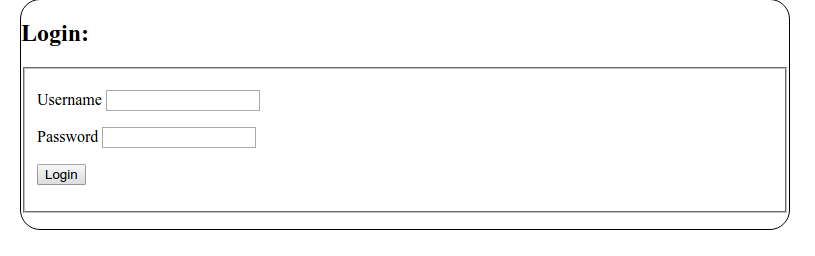
\includegraphics{img/loginscreen.png}
\caption{Bejelentkező felület\label{login}}
\end{figure}

Ha bejelentkeztünk, a böngésző oldalra dob az alkalmazás, és
lehetőségünk nyílik rendeléseket is feladni (\ref{browse}. ábra).

\begin{figure}[H]
\centering
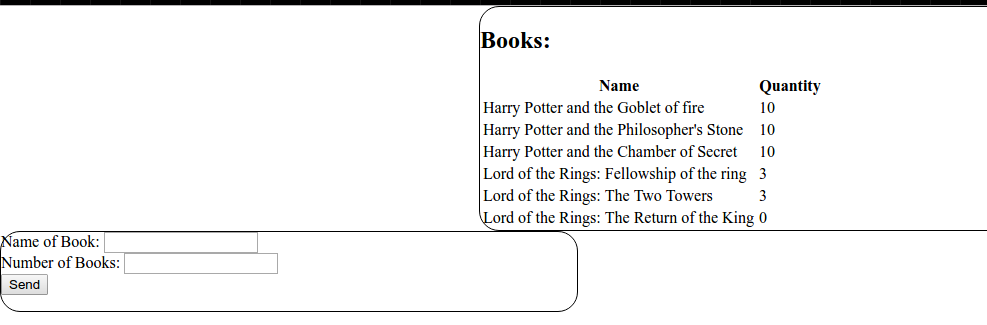
\includegraphics{img/browsescreen.png}
\caption{Böngésző felület\label{browse}}
\end{figure}

A háttérben minden kérésünkre a szolgáltatások között kommunikáció indul
meg, és a különböző funkciók esetén más-más szolgáltatás kiszolgáló
kódja indul el.

\section{Folytonos integráció
elkészítése}\label{folytonos-integruxe1ciuxf3-elkuxe9szuxedtuxe9se}

A folytonos integrációt támogató keretrendszerek közül a Jenkins-t
választottam, mivel ez a legelterjedtebb nyílt forrású eszköz, amivel
képes vagyok véghez vinni a feladatokat.

\subsection{Jenkins}\label{jenkins}

A Jenkins egy olyan folytonos integrációt támogató keretrendszer, aminek
a Java implementációja lehetővé teszi, hogy bármely, az eszközhöz
beregisztrált gépen futtassunk tetszőleges kódot. Ahhoz, hogy ezeket a
kódokat futtassuk, egy jól struktúrált végrehajtási rendszert
implementál, aminek a következők a részei:

\begin{itemize}
\tightlist
\item
  Jenkins: A Jenkins maga a legnagyobb egység, ami az összes
  végrehajtandó feladatot tartalmazza, struktúrálja, és konfigurálhatóvá
  teszi a felhasznált plugin-eket, autentikációt, és mindent ami a
  feladatokhoz tartozhat.
\item
  View: A feladatok egy jól struktúrált egysége.
\item
  Job: Ez a feladatok implementációja, minden ilyen elem tetszőleges
  mennyiségű végrehajtandó feladatot tartalmaz, képes más Job-ok
  hívására, és a plugin-ek használatával gyakorlatilag bármilyen
  feladatot képes elvégezni (csomagolást futtat, java forrásokat fordít
  maven-nel, vagy Docker konténereket vezérel, stb.).
\item
  Build: Ez az egység egy Job egyszeri futását jelenti, ehhez tartozik
  egy azonosító, ami az adott futtatást megkülönbözteti, a futtatás
  paraméterei, környezeti változói, és egy olyan szeparált környezet
  (workspace), amiben a feladatokat végrehajtja.
\end{itemize}

Ahhoz hogy megcsinálhassam az alkalmazásom fejlesztését támogató
keretrendszert, ahhoz Job-kat kellett létrehoznom, amik végrehajtották a
szoftverrel kapcsolatos feladatokat.

\subsection{Pipeline Job}\label{pipeline-job}

A Pipeline Job egy olyan Jenkins 2.0-ban elérhető feladat fajta, ami
képes egységbe szervezni a feladatokat, és levezényelni a közös
futásukat. A legtöbb folytonos integrációt támogató rendszerben egy
rövidebb, hosszabb munkafolyamatot kell lebonyolítani, aminek a pipeline
nevet adta a Jenkins, mivel az egyes feladatok futtatásai az előzetes
futások eredményétől függenek, ami annyit jelent, hogy például a
telepítési fázis függ a fordítási fázis artifact-jaitól.

A Jenkins 2.0-ban megjelenő Pipeline Job-hoz tartozik egy új leíró nyelv
is, amit Pipline szkriptnek neveznek. Lehetőség van fájlban tárolni a
konfigurációt, amit Jenkinsfile néven lehet menteni. A Dockerfile-hoz
hasonlóan ez is a működést írja le, és Pipeline szkriptet tartalmaz.

\begin{verbatim}
...
node {
    echo 'Running '+jobName+' job'
    build job: jobName
}
...
\end{verbatim}

A fenti részlet egy olyan Pipline szkriptet mutat, amiben egy bizonyos
feladatot akarunk futtatni. A `node' kulcsszó jelzi a gépet amin
futtatni akarjuk a feladatot, aminek ha nem adunk meg semmit, akkor
tetszőleges helyen fut le. A zárójelek között leírt utasítások pedig
megmondják, mi történjen azon a végponton. Egy utasítás lehet bármi amit
egy Jenkins álltal alapból támogatott Job esetén beállíthatnánk, de ezek
a parancsok inkább arra vannak kiélezve, hogy a feladatok közötti
kapcsolatot leírják. Az egyik ilyen parancs az \textbf{echo} amivel
kiírhatunk a futtatás során üzeneteket a console kimenetre. Másik
utasítás, a \textbf{build job}, amivel elindíthatunk egy `Build'-et. Az
alábbi példában egy fázis definiálása látható.

\begin{verbatim}
stage 'Deploy'
echo 'Deploying services ...'
build job: 'deploy-services'
\end{verbatim}

Egy fázis definiálása során egy képzeletbeli egységet alkotunk, ami
Job-ok, illetve parancsok futtatását tartalmazza. Új fázist a
\textbf{stage} kulcsszóval definiálhatunk, és az utána írt utasítások
mind a fázis részeként fognak megjelenni.

Az általam implementált Pipeline Job, tartalmaz egy `Build', egy
`Deploy', egy `Test', és egy `Cleanup' fázist. Az alábbi ábrán látható a
Jenkins-beli feladathoz tartozó összefoglaló nézet, ahol láthatók a Job
futtatásai:

\begin{figure}[H]
\centering
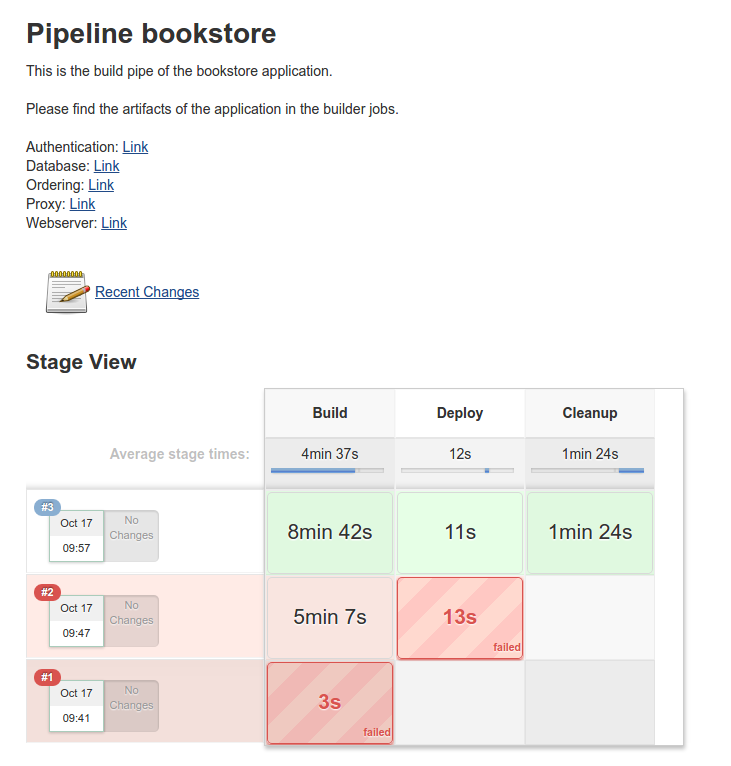
\includegraphics{img/pipeline-job.png}
\caption{Pipline Job a mikroszolgáltatások támogatásához}
\end{figure}

A képen látható, hogy hogyan is választja szép a fázisokat a Pipiline
Job, és hogy hogyan lehet kategorizálni a feladatok megívását. Az első
`Build' fázis mögött például 5 darab fordító feladat meghívását
tartalmazza, ami azt jelenti, hogy minden szolgáltatást külön fordít le
és készíti el a hozzá tartozó Docker image-et.

\subsection{Jenkins Job-ok a
keretrendszerhez}\label{jenkins-job-ok-a-keretrendszerhez}

Az előző fejezetben már látható volt, hogy van egy egész folyamatot
vezénylő Pipeline Job, amivel az összes folyamatot irányítom. Minden
fázishoz tartozik legalább egy másik Job, amiben leírtam, hogy pontosan
mit is kell csinálni abban a munkafolyamatban. A következő Job-okat
hoztam létre:

\begin{itemize}
\tightlist
\item
  build-auth-service: Autentikációs szolgáltatás elkészítése, ami egy
  Docker image-et készít.
\item
  build-database-service: Adatbázis szolgáltatás elkészítése, ami egy
  Docker image-et készít.
\item
  build-order-service: Megrendelés szolgáltatás elkészítése, ami Maven
  build segítségével elkészíti a Java programot, és egy Docker image-et
  készít.
\item
  build-proxy-service: Proxy szolgáltatás elkészítése, ami egy Docker
  image-et készít.
\item
  build-webserver-service: Böngészés szolgáltatás elkészítése, ami egy
  Docker image-et készít.
\item
  cleanup-services: Letörli a futó konténereket, és eltünteti a régi
  image-eket a Docker-ből.
\item
  deploy-services: Alkalmazás indítása, avagy a szolgáltatásokhoz
  tartozó konténerek indítása, hozzá tartozó hálózat elkészítésével.
\item
  test-services: Tesztek futtatása, amely az alkalmazás funkcionalitását
  teszteli.
\end{itemize}

\begin{figure}[H]
\centering
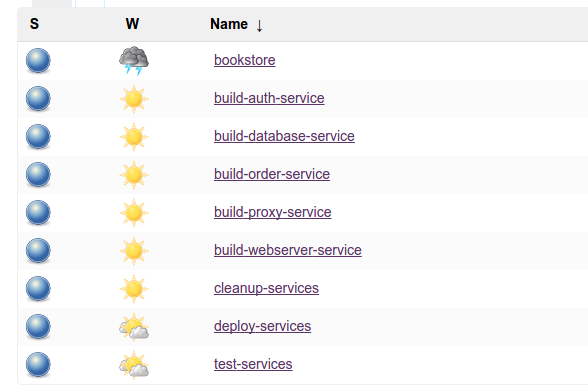
\includegraphics{img/job-view.png}
\caption{Jenkins Job-ok listája}
\end{figure}

\subsection{Job Konfigurációk}\label{job-konfiguruxe1ciuxf3k}

Vannak bizonyos beállítások, amik minden létrehozott Job-ra egyformák,
mivel egy közös verziókezelő eszközből, a GitHub-ból vette a
forrásfájlokat minden Job. Az ehhez tartozó beállításokat az
\ref{github-conf}. ábra mutatja.

\begin{figure}[H]
\centering
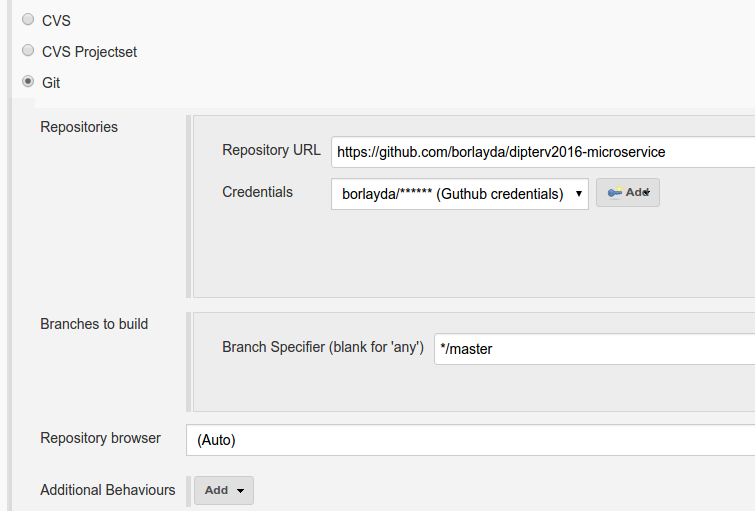
\includegraphics{img/github-config.png}
\caption{GitHub beállítások\label{github-conf}}
\end{figure}

Ez a konfiguráció azt mondja meg, hogy honnan töltse le a forrásokat a
Jenkins, és milyen branch tartalmát akarom felhasználni. Van egy
beállítás az autentikáció lebonyolítására is, ami a Jenkins-en belül egy
felhasználónév jelszó pár, amit felhasználva a Jenkins tudja használni a
GitHub-ot. Ezt a párost globálisan lehet megadni a Jenkins-nek, amit a
\emph{Jenkins/Credentials} fülön keresztül érhetünk el.

Másik mindenhol beállított tulajdonság a konkurens futtatás beállítása,
ami azt jelenti, hogy egy feladat többször is futtatható egy időben.
Feltételezve, hogy a Job-ok külön gépeken futnak, lehetséges, hogy több
példány is fusson belőlük.

Amiben minden feladat különbözik az a futtatott kód. Minden futtatandó
kódhoz készítettem egy szkriptet amit meghívhatok a Jenkins-ből. Egy
ilyen Jenkins beállítás a \ref{script-run}. ábrán látható.

\begin{figure}[H]
\centering
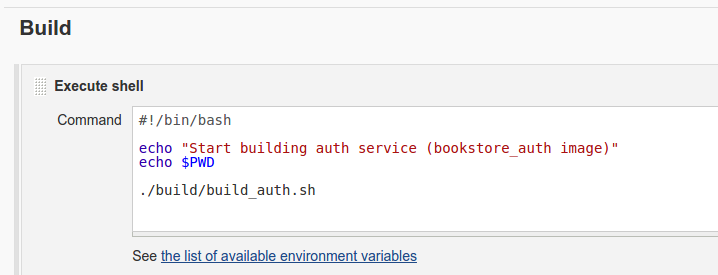
\includegraphics{img/script-run.png}
\caption{Szkript futtatása\label{script-run}}
\end{figure}

A fordító Job-ok esetén egy artifact is keletkezik, ami az adott
fordításhoz kapcsolódóan lesz lementve. A beállítást a \ref{archive}.
ábra mutatja.

\begin{figure}[H]
\centering
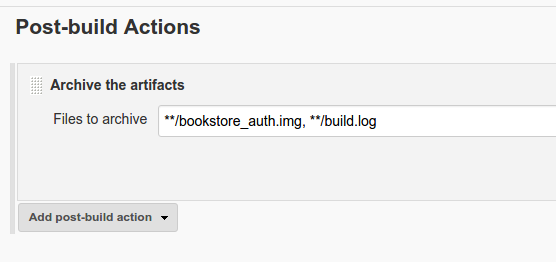
\includegraphics{img/archive.png}
\caption{Archiválás beállítása\label{archive}}
\end{figure}

Az elmentet Docker image-ek letölthetők a Jenkins-ből minden futtatás
után, így könnyen reprodukálható bármelyik futás, illetve könnyen
kiadható bármelyik verzió.

\chapter{Értékelés}\label{uxe9rtuxe9keluxe9s}

Megismertem a mikroszolgáltatásokra épülő architektúrák tervezési
módját, illetve a fejlesztésével, és karbantartásával kapcsolatos
nehézségeket. Elkészítettem egy minta alkalmazást, ami képes szimulálni
egy könyvesbolt működését, és ezt az alkalmazást mikroszolgáltatásokra
építettem. Az alkalmazás fejlesztéséhez és teszteléséhez készítettem egy
folytonos integrációt támogató keretrendszert, amivel megmondhatjuk,
hogy a változtatások jól működnek-e.

\section{Tovább fejlesztési
javaslatok}\label{tovuxe1bb-fejlesztuxe9si-javaslatok}

A minta alkalmazásban rengeteg lehetőség van a továbbfejlesztés
szempontjából. Lehet hozzá fejleszteni további funkciókat, mint a
regisztráció, keresés, vagy adminisztratív funkciók (új könyv bevitele,
készlet frissítése, stb.). A jelenlegi funkciókat is lehet tovább
fejleszteni jobb autentikációs módszerrel, szebb böngésző felülettel,
vagy árral összefűzött vásárlással. Nem csak a funkcionális
lehetőségeket érdemes kibővíteni, hanem a használhatóságot, és a
felügyeleti eszközöket, mivel monitorozás, közös log kezelés, és
skálázási lehetőségek még nincsenek az alkalmazásba építve. Sok előnnyel
járhat, ha valódi teljes hardver és szoftver virtualizációt használunk,
mivel a Docker konténerek használata körülményes lehet, és nem is igazán
stabil, ha egy gépnek kell több konténert futtatni.

Ami a folytonos integrációt támogató keretrendszert illeti, lehetőség
van a pipeline bővítésére, amit egy új funkció implementálása maga után
vonna, vagy automatikusan indíthatóvá tehető az egész verifikációs
folyam egy Jenkins pluginnel, ami a verziókezelővel együttműködve minden
új változtatásra elindíthatja a pipeline-t. Új feladatokat is hozzá
lehet fejleszteni, amik a kód minőségét javítják, és a céljuk, hogy
összeszedett jól dokumentált kód készüljön. Egy ilyen ellenőrzés lehetne
a Python fájlok formai kiértékelése, ami lehetséges a pylint programmal.

\section{Problémák, Kritika}\label{probluxe9muxe1k-kritika}

A feladat elkészítése közben több probléma is felmerült, ami könnyen
lehet fejlesztés közben blokkoló tényező. A legnagyobb probléma a Docker
image-ek készítésénél volt, mivel a Docker által készített image-ek
gyakran változnak, és a visszafelé kompatibilitás nem teljesül 2 verzió
között. A témával kapcsolatban találtam egy cikket\citep{docker-is-bad},
ami kifejti, hogy pontosan hol is vannak a hibák a Docker fejlesztési
stratégiában, amit a felhasználók észrevehetnek.

Ezzel szembesültem én is, amikor fejlesztettem az adatbázis
szolgáltatást, vagy a megrendelés szolgáltatását. A felhasznált
\textbf{ubuntu} image mögött a csomagok dinamikusan változnak, és két
fordítási folyamat között is előfordul, hogy ugyan azon a néven más-más
csomagot telepítünk. Az adatbázis kezelő esetén a MySQL csomag lett
újabb, és egy nem várt felhasználónév jelszó párost kért, mivel többé
már nem volt telepítés utáni alapértelmezett felhasználó. A probléma
ugyan nem volt jelentős, de minden szolgáltatást érintett, és éppen
ezért hosszabb időt vett igénybe a javítása. A megrendelés esetén a
\textbf{centos} alap image változott meg, és nem lehetett egyáltalán
szolgáltatást indítani a konténer belsejéből. Sajnálatos módon a
megoldás az alap image cseréje volt.

\section{Hol használható}\label{hol-hasznuxe1lhatuxf3}

Az elkészített folytonos integrációt támogató keretrendszer szinte
minden mikroszolgáltatás alapú alkalmazás támogatásához felhasználható,
mivel a folyamat amit implementál, és a szkriptek, amikkel a
fordításokat lebonyolítom, és a telepítést végzem, könnyen
megváltoztathatók bármely más alkalmazás kiszolgálására. A minta
alkalmazás nem lenne képes valós könyvesbolt vásárlásának irányítására,
azonban nagyon jó mintául szolgál a fejlesztés bemutatására, mivel
tartalmaz komplex szolgáltatásokat, amik önállóan megtalálják egymást,
és elég egyszerű, hogy tetszőlegesen továbbfejleszthető legyen.

\listoffigures

\bibliography{bibliography}


\appendix

\chapter{Függelék}\label{fuxfcggeluxe9k}

\section{\texorpdfstring{Dockerfile-ok\label{appendix-dockerfile}}{Dockerfile-ok}}\label{dockerfile-ok}

\subsection{Autentikáció}\label{autentikuxe1ciuxf3}

Dockerfile.auth.service

\begin{verbatim}
FROM ubuntu
MAINTAINER Borlay Dániel <borlay.daniel@gmail.com>

ENV CONSUL_DIR /usr/share/consul

# Install Service
COPY auth-service.py /usr/sbin/auth-service.py
RUN apt-get -y update && \
    apt-get -y install \
        bash \
        iputils-ping \
        python-oauth \
        python-mysqldb \
        python \
        python-flask && \
    chmod +x /usr/sbin/auth-service.py

# Install consul
COPY consul consul-template /usr/bin/
RUN chmod +x /usr/bin/consul && \
    chmod +x /usr/bin/consul-template && \
    mkdir -p /etc/consul.d
COPY auth.json /etc/consul.d/auth.json

# Install entry point
COPY init /usr/sbin/init-auth
RUN chmod +x /usr/sbin/init-auth

ENTRYPOINT /bin/bash /usr/sbin/init-auth

EXPOSE 8081 8301 8302 8500 8400
\end{verbatim}

\subsection{Proxy}\label{proxy}

Dockerfile.proxy.service

\begin{verbatim}
FROM haproxy
MAINTAINER Borlay Dániel <borlay.daniel@gmail.com>

ENV CONSUL_DIR /usr/share/consul

# Install Service
COPY proxy.sh /usr/sbin/proxy.sh
RUN apt-get -y update && \
    apt-get -y --force-yes install haproxy iputils-ping && \
    chmod +x /usr/sbin/proxy.sh
COPY haproxy.cfg /etc/haproxy/haproxy.cfg

# Install consul
COPY consul consul-template /usr/bin/
RUN mkdir -p /etc/consul.d && \
    chmod +x /usr/bin/consul && \
    chmod +x /usr/bin/consul-template
COPY proxy.json /etc/consul.d/proxy.json

# Install entry point
COPY init /usr/sbin/init-proxy
RUN chmod +x /usr/sbin/init-proxy

ENTRYPOINT /bin/bash /usr/sbin/init-proxy

EXPOSE 8080 8301 8302 8500 8400
\end{verbatim}

\subsection{Adatbázis}\label{adatbuxe1zis}

Dockerfile.database.service

\begin{verbatim}
FROM ubuntu
MAINTAINER Borlay Dániel <borlay.daniel@gmail.com>

USER root
ENV CONSUL_DIR /usr/share/consul

# Install Service
COPY database.sh /usr/sbin/database.sh
COPY auth_init.sql bookstore_init.sql /tmp/
RUN apt-get -y update && \
    /bin/bash -c "debconf-set-selections \
<<< 'mysql-server mysql-server/root_password password root'" && \
    /bin/bash -c "debconf-set-selections \
<<< 'mysql-server mysql-server/root_password_again password root'" && \
    apt-get -y install mysql-server \
        iputils-ping \
        mysql-client && \
    chmod +x /usr/sbin/database.sh

# Install consul
COPY consul consul-template /usr/bin/
RUN mkdir -p /etc/consul.d && \
    chmod +x /usr/bin/consul && \
    chmod +x /usr/bin/consul-template
COPY database.json /etc/consul.d/database.json

# Install entry point
COPY init /usr/sbin/init-db
RUN chmod +x /usr/sbin/init-db && \
    sed -i 's/bind-address.*=.*/bind-address = 0.0.0.0/g' \
        /etc/mysql/mysql.conf.d/mysqld.cnf

ENTRYPOINT /bin/bash /usr/sbin/init-db

EXPOSE 3306 8301 8302 8500 8400
\end{verbatim}

\subsection{Vásárlás}\label{vuxe1suxe1rluxe1s}

Dockerfile.order.service

\begin{verbatim}
FROM tomcat
MAINTAINER Borlay Dániel <borlay.daniel@gmail.com>

ENV CONSUL_DIR /usr/share/consul

# Install Service
RUN sed -i 's/8080/8888/g' /usr/local/tomcat/conf/server.xml && \
    sed -i 's/<Connector /<Connector address="0.0.0.0" \
        /g' /usr/local/tomcat/conf/server.xml
COPY target/ReserveRESTJerseyExample-0.0.2-SNAPSHOT.war \
    /usr/local/tomcat/webapps/order.war

# Install consul
COPY consul consul-template /usr/bin/
RUN mkdir -p /etc/consul.d && \
    chmod +x /usr/bin/consul && \
    chmod +x /usr/bin/consul-template
COPY order.json /etc/consul.d/order.json

# Install entry point
COPY init /usr/local/sbin/init-order
RUN chmod +x /usr/local/sbin/init-order

ENTRYPOINT /bin/bash /usr/local/sbin/init-order

EXPOSE 8888 8301 8302 8500 8400
\end{verbatim}

\subsection{Webkiszolgáló
(böngészés)}\label{webkiszolguxe1luxf3-buxf6nguxe9szuxe9s}

Dockerfile.web.service

\begin{verbatim}
FROM ubuntu
MAINTAINER Borlay Dániel <borlay.daniel@gmail.com>

ENV CONSUL_DIR /usr/share/consul

# Install Service
COPY webserver.sh /usr/sbin/webserver.sh
RUN apt-get -y update && \
    apt-get -y install apache2 php \
        libapache2-mod-php \
        php-mysql \
        curl \
        iputils-ping \
        php-curl && \
    chmod +x /usr/sbin/webserver.sh
COPY index.html main.css login.php store.php order.php /var/www/html/

# Install consul
COPY consul consul-template /usr/bin/
RUN mkdir -p /etc/consul.d && \
    chmod +x /usr/bin/consul && \
    chmod +x /usr/bin/consul-template
COPY web.json /etc/consul.d/web.json

# Install entry point
COPY init /usr/sbin/init-web
RUN chmod +x /usr/sbin/init-web

ENTRYPOINT /bin/bash /usr/sbin/init-web

EXPOSE 80 443 8301 8302 8500 8400
\end{verbatim}

\section{Szkriptek}\label{szkriptek}

\subsection{Futtatáshoz}\label{futtatuxe1shoz}

\subsubsection{\texorpdfstring{Fordítás\label{appendix-build}}{Fordítás}}\label{forduxedtuxe1s}

build\_\{service\}.sh

\begin{verbatim}
#!/bin/bash

<SERVICE>_SERVICE_HOME=services/<SERVICE>
<SERVICE>_SERVICE_DOCKERFILE=Dockerfiles/Dockerfile.<SERVICE>.service
<SERVICE>_SCRIPT_DIR=scripts/<SERVICE>
<SERVICE>_CONF_DIR=conf/<SERVICE>
<SERVICE>_IMAGE_NAME=bookstore_<SERVICE>

CONSUL_BASE=https://releases.hashicorp.com
CON_VER=0.7.0/consul_0.7.0_linux_386.zip
CONSUL_URL=${CONSUL_BASE}/consul/${CON_VER}
TEMP_VER=0.16.0/consul-template_0.16.0_linux_386.zip
CONSULT_URL=${CONSUL_BASE}/consul-template/${TEMP_VER}

pushd ..
if [[ ! -e consul ]]; then
    echo "Get Consul script from Internet"
    wget ${CONSUL_URL} && unzip consul_0.7.0_linux_386.zip
fi

if [[ ! -e consul-template ]]; then
    echo "Get consul-template script from Internet"
    wget ${CONSULT_URL} && unzip consul-template_0.16.0_linux_386.zip
fi

echo "Create <SERVICE> service for bookstore ..."
echo " - Create directory for Docker data"
mkdir -p ${<SERVICE>_SERVICE_HOME}
echo " - Move Dockerfile to data directory"
cp ${<SERVICE>_SERVICE_DOCKERFILE} ${<SERVICE>_SERVICE_HOME}/Dockerfile
echo " - Move script files to data directory"
cp -R ${<SERVICE>_SCRIPT_DIR}/* ${<SERVICE>_SERVICE_HOME}/
echo " - Move config files to data directory"
cp -R ${<SERVICE>_CONF_DIR}/* ${<SERVICE>_SERVICE_HOME}/
echo " - Move consul to data directory"
cp consul ${<SERVICE>_SERVICE_HOME}/
cp consul-template ${<SERVICE>_SERVICE_HOME}/
echo " - Building Docker image"
docker build -t ${<SERVICE>_IMAGE_NAME} \
    ${<SERVICE>_SERVICE_HOME} &> ${<SERVICE>_SERVICE_HOME}/build.log
echo " - Save image"
docker save \
    --output ${<SERVICE>_SERVICE_HOME}/${<SERVICE>_IMAGE_NAME}.img \
    ${DATABASE_IMAGE_NAME}

echo "<SERVICE> service has been created!"
popd
\end{verbatim}

\subsubsection{\texorpdfstring{Futtatás\label{appendix-runner}}{Futtatás}}\label{futtatuxe1s}

run\_containers.sh

\begin{verbatim}
#!/bin/bash

services="database webserver order auth proxy"

docker network create bookstore

for service in ${services}
do
    echo "Start ${service} service ..."
    docker run -d --name "${service}" \
               -h "${service}" \
              --net=bookstore bookstore_${service}
done
\end{verbatim}

\subsubsection{\texorpdfstring{Tisztogatás\label{appendix-cleanup}}{Tisztogatás}}\label{tisztogatuxe1s}

clean\_docker.sh

\begin{verbatim}
#!/bin/bash

services="database webserver proxy order auth"

docker stop $(docker ps -a | awk '/bookstore/ {print $1}')
docker rm $(docker ps -a | awk '/bookstore/ {print $1}')

for service in ${services}
do
    echo "Delete ${service} image"
    docker rmi bookstore_${service}
done

if [ -d services ]; then
    rm -rf services
fi
docker network rm bookstore

if [ -e consul ]; then
    rm -rf consul*
fi
\end{verbatim}

\subsection{Szolgáltatásokhoz}\label{szolguxe1ltatuxe1sokhoz}

\subsubsection{\texorpdfstring{Init
szkript\label{appendix-starter}}{Init szkript}}\label{init-szkript}

\begin{verbatim}
#!/bin/bash

IP_ADDR=$(hostname -I)
MASK=${IP_ADDR%.*}

while true; do
    FOUND=false
    for ADDR in $(seq 1 255); do
        echo "${MASK}.${ADDR}  ${IP_ADDR}"
        [[ "${MASK}.${ADDR}" == "${IP_ADDR}" ]] && continue
        ping -c 1  "${MASK}.${ADDR}"
        [ $? -eq 0 ] || continue
        echo "Try consul with ${MASK}.${ADDR}"
        consul agent -server \
                     -join "${MASK}.${ADDR}" \
                     -datacenter "bookstore" \
                     -data-dir "${CONSUL_DIR}" \
                       > /var/log/bookstore-consul.log &
        sleep 10
        cat /var/log/bookstore-consul.log
        if ps ax | grep -v grep | grep "consul" > /dev/null; then
            echo "Consul could run!!!"
            FOUND=true
            break
        fi
    done
    echo "${FOUND}"
    if [[ "${FOUND}" == "true" ]]; then
        break
    fi
done
<service>.sh
\end{verbatim}

\subsubsection{\texorpdfstring{Böngészés
kódjai\label{appendix-http}}{Böngészés kódjai}}\label{buxf6nguxe9szuxe9s-kuxf3djai}

Login oldal:

\begin{verbatim}
<?php

if(!isset( $_POST['username'], $_POST['password']))
{
    echo 'Please enter a valid username and password';
}
else
{
    $username = filter_var($_POST['username'], FILTER_SANITIZE_STRING);
    $password = filter_var($_POST['password'], FILTER_SANITIZE_STRING);

    $ch = curl_init();
    curl_setopt($ch, CURLOPT_RETURNTRANSFER, true);
    curl_setopt($ch, CURLOPT_URL,
        "http://auth:8081/auth/{$username}/{$password}"
    );
    $output = curl_exec($ch);
    $info = curl_getinfo($ch);
    if ($output === false || $info['http_code'] != 200) {
        header("Location: /login.php");
        die();
    }
    else {
        header("Location: /store.php");
        die();
    }
    curl_close($ch);
}
?>
\end{verbatim}

Könyveket megjelenítő oldal:

\begin{verbatim}
<html>
<head>
<title>Bookstore Microservice</title>
<link rel="stylesheet" type="text/css" href="main.css">
</head>
<body>

<div id="storeBox">
<h2>Books:</h2>

<table>
  <tbody>
    <tr><th>Name</th><th>Quantity</th></tr>

    <?php
      $servername = "database";
      $username = "store";
      $password = "store";
      $dbname = "bookstore";

      // Create connection
      $conn = new mysqli($servername, $username, $password, $dbname);
      // Check connection
      if ($conn->connect_error) {
          die("Connection failed: " . $conn->connect_error);
      }

      $sql = "SELECT * FROM store";
      $result = $conn->query($sql);

      if ($result->num_rows > 0) {
          // output data of each row
          while($row = $result->fetch_assoc()) {
              echo "<tr><td>" . $row["book_name"]. \
                "</td><td> " . $row["count"]. "</td></tr>";
          }
      } else {
          echo "0 results";
      }
      $conn->close();
    ?>

  </tbody>
</table>
</div>
<div id="orderBox">
<form action="order.php" method="post">
    <span>Name of Book: </span>\
        <input type="text" name="nameOfBook" /><br/>
    <span>Number of Books: </span>\
        <input type="text" name="numberOfBooks"/><br/>
    <input type="submit" name="send" value="Send"/>
</form>
</div>

</body>
</html>
\end{verbatim}

\subsubsection{\texorpdfstring{Adatbázis
inicializálás\label{appendix-database}}{Adatbázis inicializálás}}\label{adatbuxe1zis-inicializuxe1luxe1s}

Autentikáció:

\begin{verbatim}
# Add permission to databases
GRANT ALL PRIVILEGES ON authenticate.* TO 'root'@'%';
GRANT ALL PRIVILEGES ON authenticate.* TO 'root'@'localhost';
# Create Tables
CREATE TABLE user_auth
(
    user_id int NOT NULL AUTO_INCREMENT,
    username varchar(255) NOT NULL,
    password varchar(255) NOT NULL,
    credential varchar(255),
    PRIMARY KEY (user_id)
);
# Fill Tables
INSERT INTO user_auth (username, password)
VALUES ("test", "testpassword");
\end{verbatim}

Bookstore raktár:

\begin{verbatim}
# Add permission to databases
GRANT ALL PRIVILEGES ON bookstore.* TO 'root'@'%';
GRANT ALL PRIVILEGES ON bookstore.* TO 'root'@'localhost';
# Create Tables
CREATE TABLE store
(
    store_id int NOT NULL AUTO_INCREMENT,
    book_name varchar(255) NOT NULL,
    count int NOT NULL,
    PRIMARY KEY (store_id)
);
CREATE TABLE reservation
(
    reservation_id int NOT NULL AUTO_INCREMENT,
    username varchar(255) NOT NULL,
    book_name varchar(255) NOT NULL,
    count int NOT NULL,
    res_date varchar(255),
    PRIMARY KEY (reservation_id)
);
# Fill Tables
INSERT INTO store (book_name, count)
VALUES ("Harry Potter and the Goblet of fire", 10);
INSERT INTO store (book_name, count)
VALUES ("Harry Potter and the Philosopher's Stone", 10);
INSERT INTO store (book_name, count)
VALUES ("Harry Potter and the Chamber of Secret", 10);
INSERT INTO store (book_name, count)
VALUES ("Lord of the Rings: Fellowship of the ring", 3);
INSERT INTO store (book_name, count)
VALUES ("Lord of the Rings: The Two Towers", 3);
INSERT INTO store (book_name, count)
VALUES ("Lord of the Rings: The Return of the King", 0);
\end{verbatim}

\subsection{\texorpdfstring{Pipeline job
szkript\label{appendix-pipline}}{Pipeline job szkript}}\label{pipeline-job-szkript}

Pipeline job full szkript:

\begin{verbatim}
buildNames = [
    'build-auth-service',
    'build-database-service',
    'build-order-service',
    'build-proxy-service',
    'build-webserver-service'
]

def buildJobs = [:]

for (int i=0; i<buildNames.size(); ++i) {
    def buildName = buildNames[i]
    buildJobs[buildNames[i]] = {
        node {
            echo 'Running '+buildName+' build'
            build job: buildName
        }
    }
}

stage 'Build'
echo 'Building services ...'
parallel buildJobs
stage 'Deploy'
echo 'Deploying services ...'
build job: 'deploy-services'
stage 'Test'
echo 'Testing services ...'
build job: 'test-services'
stage 'Cleanup'
echo 'Cleaning up services ...'
build job: 'cleanup-services'
\end{verbatim}

\subsection{\texorpdfstring{Proxy\label{appendix-template}}{Proxy}}\label{proxy-1}

Proxy konfigurációs minta:

\begin{verbatim}
global
    log 127.0.0.1 local1 notice
    chroot /var/lib/haproxy
    stats socket /run/haproxy/admin.sock mode 660 level admin
    stats timeout 30s
    user haproxy
    group haproxy
    daemon

defaults
    log     global
    mode    http
    option  httplog
    option  dontlognull
    timeout connect 5000
    timeout client  50000
    timeout server  50000
    errorfile 500 /etc/haproxy/errors/500.http

frontend web
    bind *:80
    mode http
    default_backend nodes

backend nodes
    mode http
    balance roundrobin{{range "app.web"}}
    service {{.ID}} {{.Address}}:{{.Port}}{{end}}

frontend database
    bind *:3306
    default_backend dbnodes

backend dbnodes
    balance roundrobin{{range "app.database"}}
    service {{.ID}} {{.Address}}:{{.Port}}{{end}}

frontend order
    bind *:8888
    default_backend onodes

backend onodes
    balance roundrobin{{range "app.order"}}
    service {{.ID}} {{.Address}}:{{.Port}}{{end}}

frontend auth
    bind *:8081
    default_backend anodes

backend anodes
    balance roundrobin{{range "app.auth"}}
    service {{.ID}} {{.Address}}:{{.Port}}{{end}}
\end{verbatim}

\end{document}
